\chapter{Déploiement de l'infrastructure IT}

%\markboth{Chapitre 2 }{Déploiement de l'infrastructure IT} %pour afficher l'entete
%\addcontentsline{toc}{chapter}{Chapitre 2 : Déploiement de l'infrastructure IT}


\section{Introduction}

Le déploiement de l'infrastructure informatique est une étape cruciale pour le de Zeta Engineering. Après avoir choisi la méthodologie en cascade, nous sommes prêts à passer à la mise en place de l'infrastructure nécessaire à la réalisation du projet. \\

Dans ce chapitre, nous détaillons les différentes étapes du déploiement de l'infrastructure IT, notamment la mise en place du réseau, la sélection des équipements matériels et logiciels. \\

Nous expliquons également les choix techniques que nous avons effectués pour répondre aux exigences de l'entreprise et assurer une infrastructure robuste et sécurisée. Tout au long de ce chapitre, nous détaillons les différentes étapes du déploiement et expliquons les raisons de nos choix techniques afin de permettre une compréhension approfondie de notre approche. \\




\section{Outils et Technologies Utilisées}

Dans cette partie, nous allons détailler les différents outils et technologies que nous avons utilisés pour établir l'infrastructure réseau IT et SI nécessaire à la mise en place.\\

Nous abordons tout d'abord le matériel que nous avons sélectionné et configuré pour répondre aux besoins de l'entreprise, dans la sous-section 2.1 "Matériel Utilisé". \\

Ensuite, nous présentons l'environnement IT que nous avons mis en place, en décrivant les différentes technologies et logiciels utilisés pour assurer une infrastructure stable, performante et sécurisée, dans la sous-section "Environnement IT".  \\

Cette présentation détaillée nous permettra de mieux comprendre les choix que nous avons effectués pour répondre aux exigences de l'entreprise et assurer une mise en œuvre réussie de notre projet. \\

\subsection{Matériel Utilisé}

Dans cette sous-section, nous présentons le matériel utilisé, notamment les commutateurs, le pare-feu et les cartes électroniques, sous forme d'un tableau comme suit.


\begin{table}[H]
\begin{center}
\begin{tabular}{|c{3cm}|c{3cm}|c{10cm}|}
\hline
\textbf{Logo}         & \textbf{Nom de l'équipement}   & \textbf{Fonctionnalité} \\
\hline
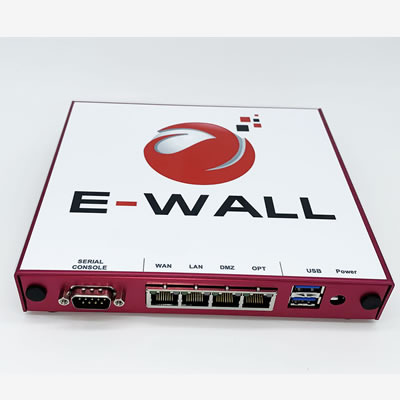
\includegraphics[width=3cm]{Images/ewall.jpg} & E-Wall Pare-Feu & Une solution de sécurité essentielle pour protéger les réseaux informatiques contre les menaces externes. Son utilisation permet de renforcer la sécurité, de contrôler le trafic réseau et de détecter les activités malveillantes, contribuant ainsi à la préservation de l'intégrité, de la confidentialité et de la disponibilité des données. \\
\hline
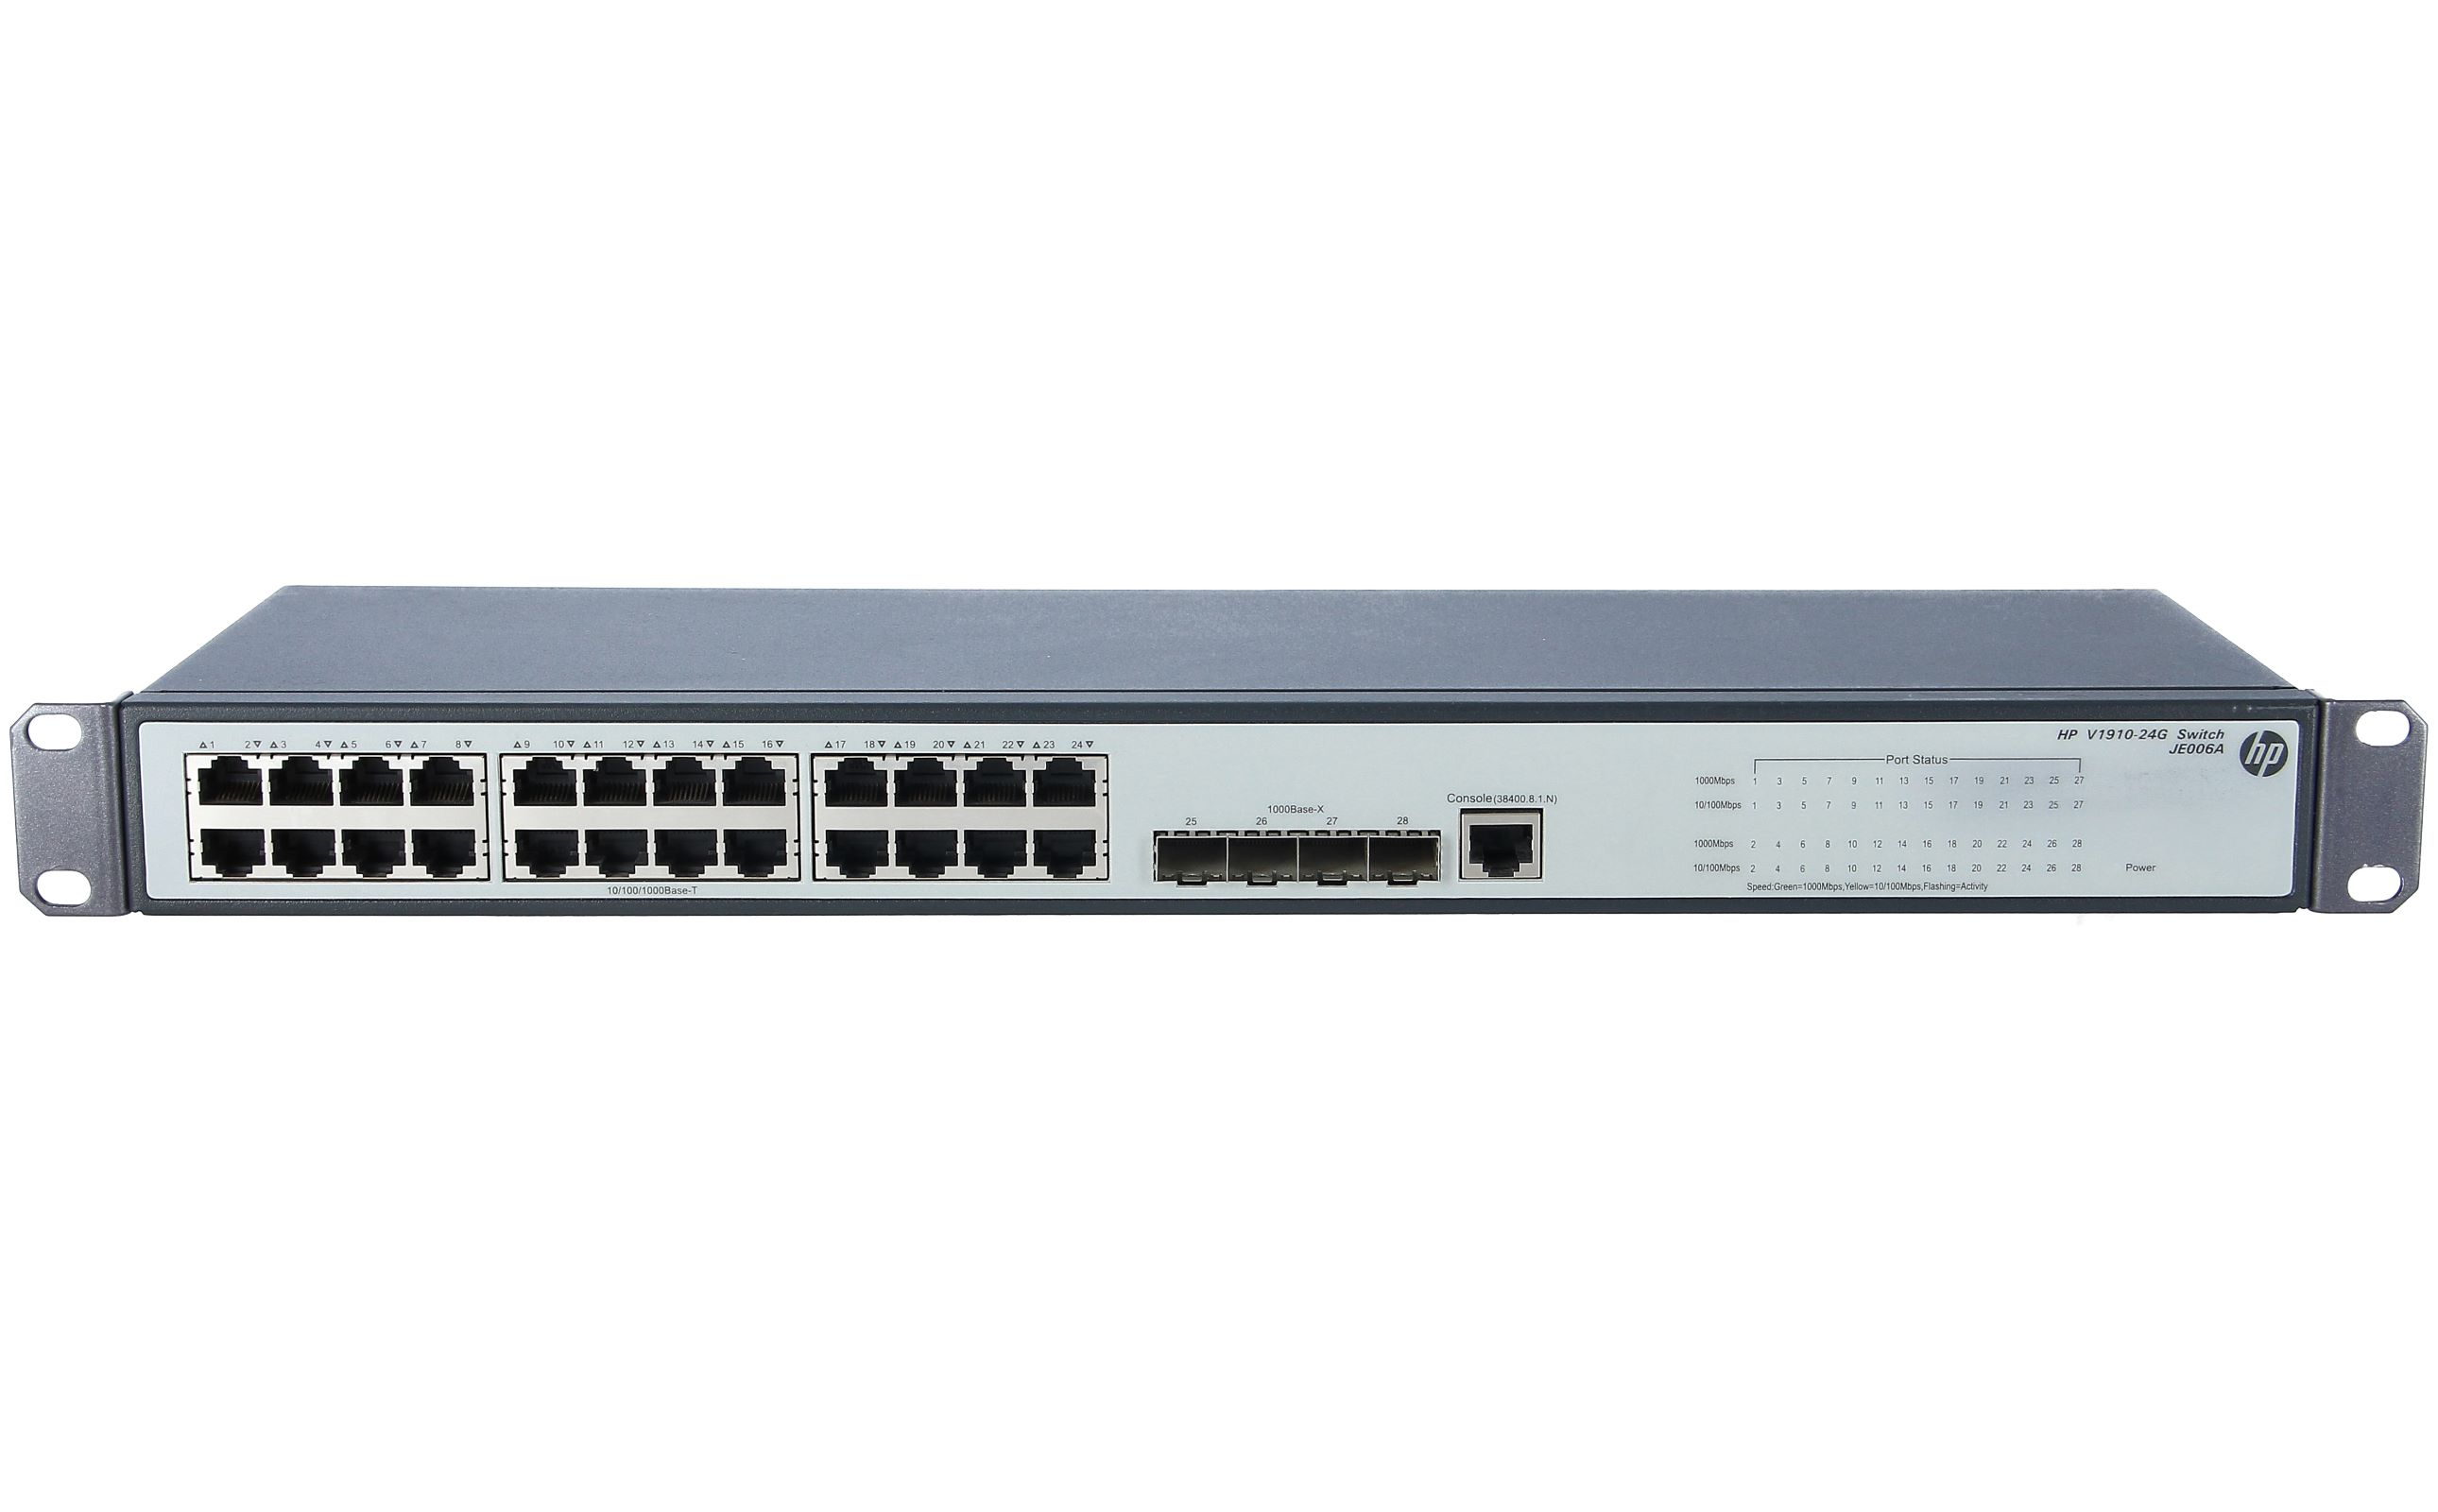
\includegraphics[width=3cm]{Images/HP1910.jpg} & Commutateurs HP1910 G24 & Un modèle de commutateur d'entreprise qui offre des fonctionnalités de gestion avancées pour les réseaux LAN. Il dispose de 24 ports Gigabit Ethernet et peut être géré via une interface web ou en ligne de commande. Il prend en charge les protocoles de gestion de réseau SNMP, RMON et LLDP, ainsi que les VLAN, le QoS, le STP et d'autres fonctionnalités de sécurité.  \\
\hline
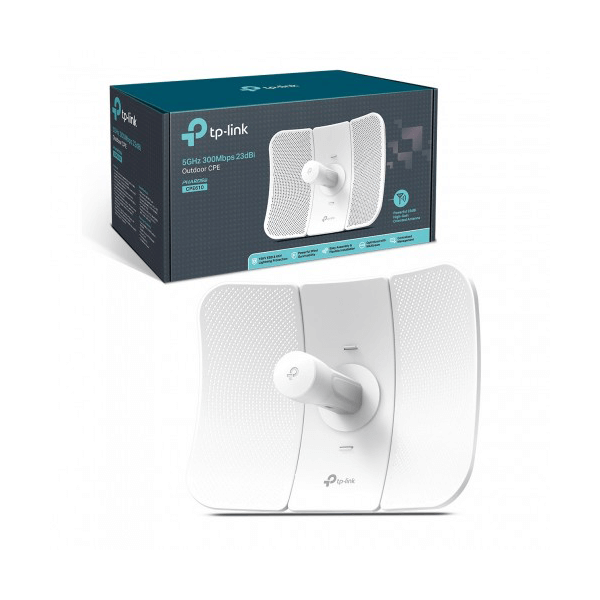
\includegraphics[width=3cm]{Images/TP-Link-CPE610-5GHz_1.png} & TP-Link CPE610 & Le TP-Link CPE610 est un point d'accès extérieur sans fil conçu pour fournir une connectivité Wi-Fi à longue portée dans des environnements extérieurs. Il utilise une antenne directionnelle à haut gain pour offrir des connexions sans fil stables et fiables sur de longues distances.  \\
\hline
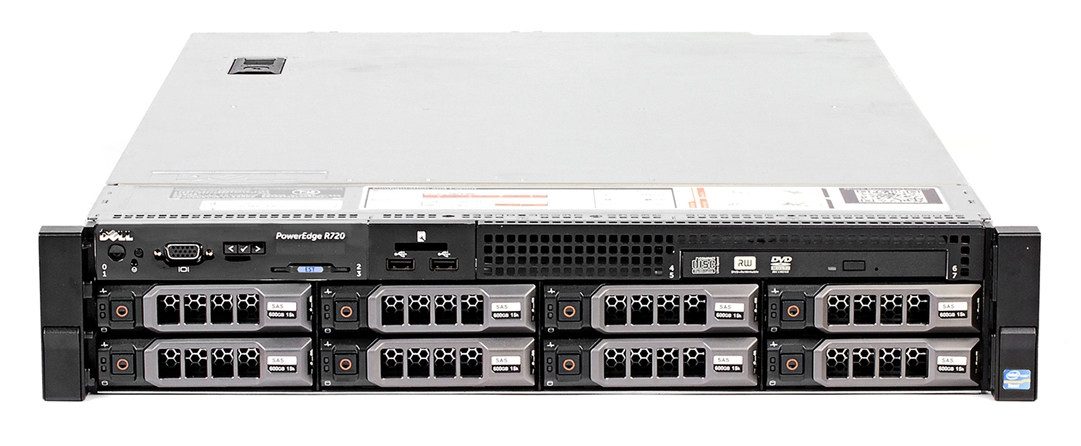
\includegraphics[width=3cm]{Images/dellr720.jpg} & Dell PowerEdge R720 & Le Dell PowerEdge R720 est un serveur rackable de haute performance, fiable et évolutif, offrant une grande capacité de stockage et de traitement de données pour les applications critiques de l'entreprise. Il est équipé de processeurs Intel Xeon E5-2600 v2 et peut prendre en charge jusqu'à 1,5 To de mémoire vive. Le PowerEdge R720 dispose également de fonctionnalités de haute disponibilité telles que les alimentations redondantes, les disques durs en miroir et les cartes réseau doubles. \\
\hline
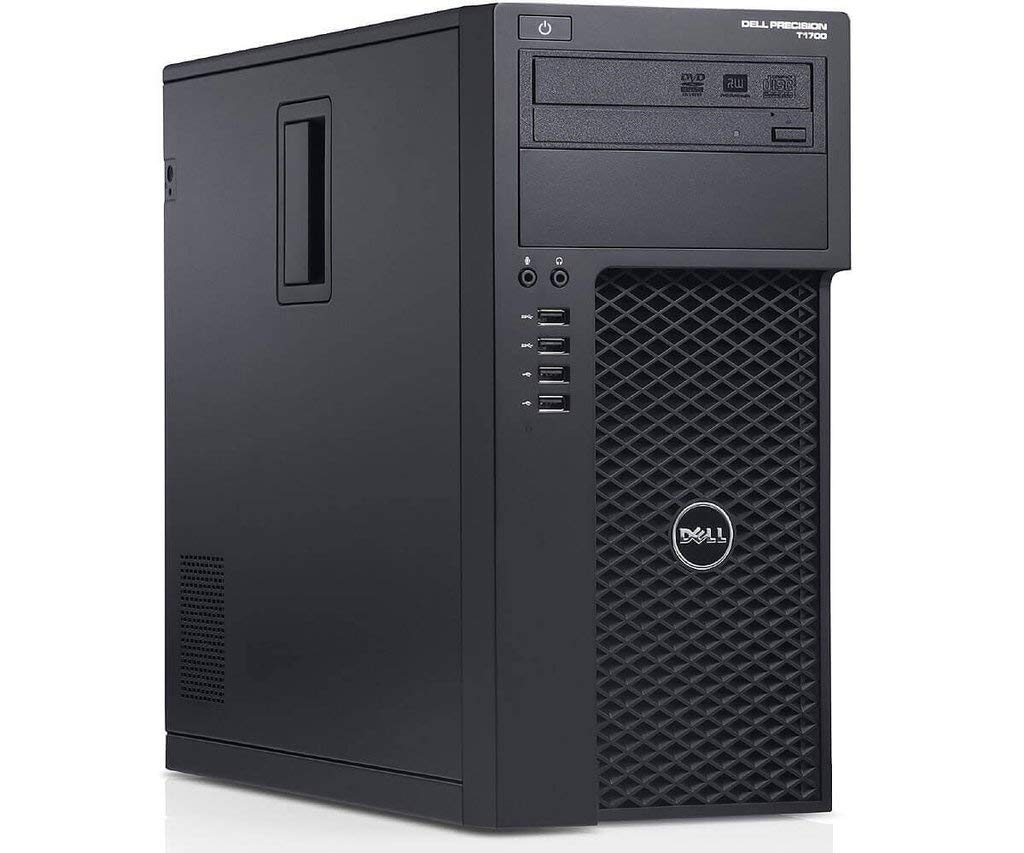
\includegraphics[width=3cm]{Images/1700Dell.jpg} & Le Dell T1700 Tower & Le Dell T1700 Tower est un modèle de serveur de bureau de la gamme Dell Precision. Il est conçu pour offrir des performances fiables et une grande stabilité pour les applications professionnelles exigeantes. Le T1700 est équipé d'un processeur Intel Core i7 et peut prendre en charge jusqu'à 32 Go de mémoire vive. \\
\hline
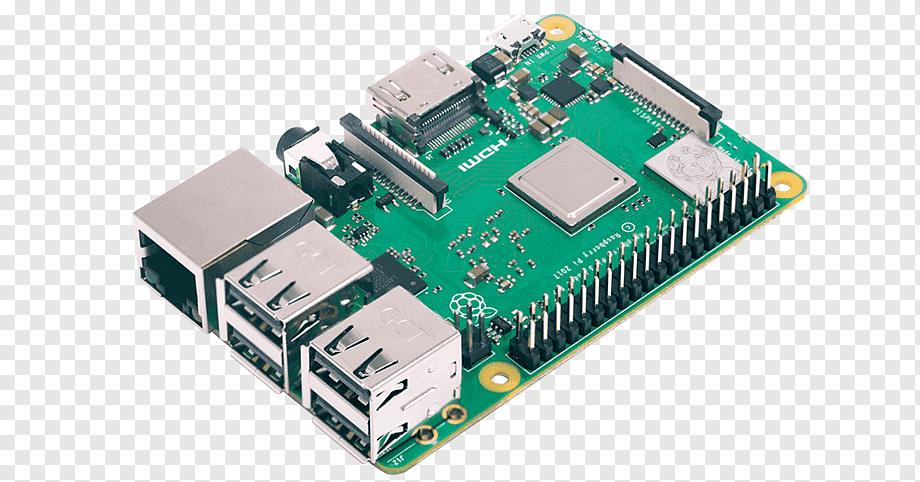
\includegraphics[width=3cm]{Images/RaspberryPi3.jpg} & Raspberry Pi B+ V1.2 & Un ordinateur monocarte (single-board computer) de la taille d'une carte de crédit, développé par la fondation Raspberry Pi. Il est équipé d'un processeur ARM Cortex-A53 quad-core à 1,4 GHz, de 1 Go de RAM, de plusieurs ports USB, d'un port Ethernet, de connecteurs audio et vidéo, et d'un slot pour carte microSD pour le stockage. Il peut être utilisé pour une grande variété de projets, notamment des serveurs, des media centers, des stations de développement, des robots, des systèmes embarqués, etc. \\
\hline
\end{tabular}
\caption{Tableau du matériel utilisées}
\label{1}
\end{center}
\end{table}



\subsection{Logiciel utilisé}

Dans cette sous-section nous présentons les logiciels utilisées comme les GNS3 et VNC Viewer pour créer notre infrastructure réseau sous forme de tableau suivant. 


\begin{table}[H]
\begin{center}
\begin{tabular}{|c{3cm}|c{3cm}|c{10cm}|}
\hline
\textbf{Logo}         & \textbf{Nom de l'équipement}   & \textbf{Fonctionnalité} \\
\hline

\includegraphics[width=3cm]{Images/Logo-GNS3.png} & GNS3 & GNS3 est un logiciel open-source de simulation de réseaux informatiques. Il permet de créer des topologies réseau virtuelles en utilisant des images de routeurs, de commutateurs et d'autres équipements réseau. \\
\hline

\includegraphics[width=3cm]{Images/Logo-VMWare.jpg}  & VMware Workstation & VMware Workstation est un logiciel de virtualisation puissant qui permet d'exécuter plusieurs systèmes d'exploitation sur une seule machine physique. Il offre la possibilité de créer et de gérer des machines virtuelles (VM) sur une plateforme hôte, ce qui permet d'exécuter plusieurs systèmes d'exploitation simultanément. VMware Workstation est disponible pour les principales plateformes telles que Windows, Linux et macOS. \\
\hline

\includegraphics[width=3cm]{Images/Logo-VNCViewer.png} & VNC Viewer & VNC Viewer est une application de bureau à distance qui permet de se connecter à un ordinateur distant et d'en contrôler l'écran et les applications à distance. Il offre la possibilité de se connecter à distance à des appareils tels que le Raspberry Pi, permettant ainsi une gestion et un contrôle pratiques de l'appareil à partir d'un autre ordinateur. \\
\hline

\includegraphics[width=3cm]{Images/Logo-IPScanner.png} & Advanced IP Scanner & Advanced IP Scanner est un outil de gestion de réseau qui permet de scanner rapidement un réseau et de trouver tous les périphériques connectés, y compris les ordinateurs, les imprimantes, les routeurs, les commutateurs, les caméras IP, etc. Il permet également de détecter les adresses IP inactives et les ports ouverts sur les périphériques.  \\
\hline

\includegraphics[width=3cm]{Images/Logo-Fritzing.png} & Fritzing & Fritzing est un logiciel de conception électronique open-source qui permet de créer des schémas électroniques, des circuits imprimés et des modèles de connexion pour des projets électroniques. Il offre une interface conviviale et intuitive, ce qui facilite la création de schémas électroniques même pour les débutants. \\
\hline
\end{tabular}
\caption{Tableau du logiciel utilisées - Partie 1}
\label{1}
\end{center}
\end{table}


\begin{table}[H]
\begin{center}
\begin{tabular}{|c{3cm}|c{3cm}|c{10cm}|}
\hline
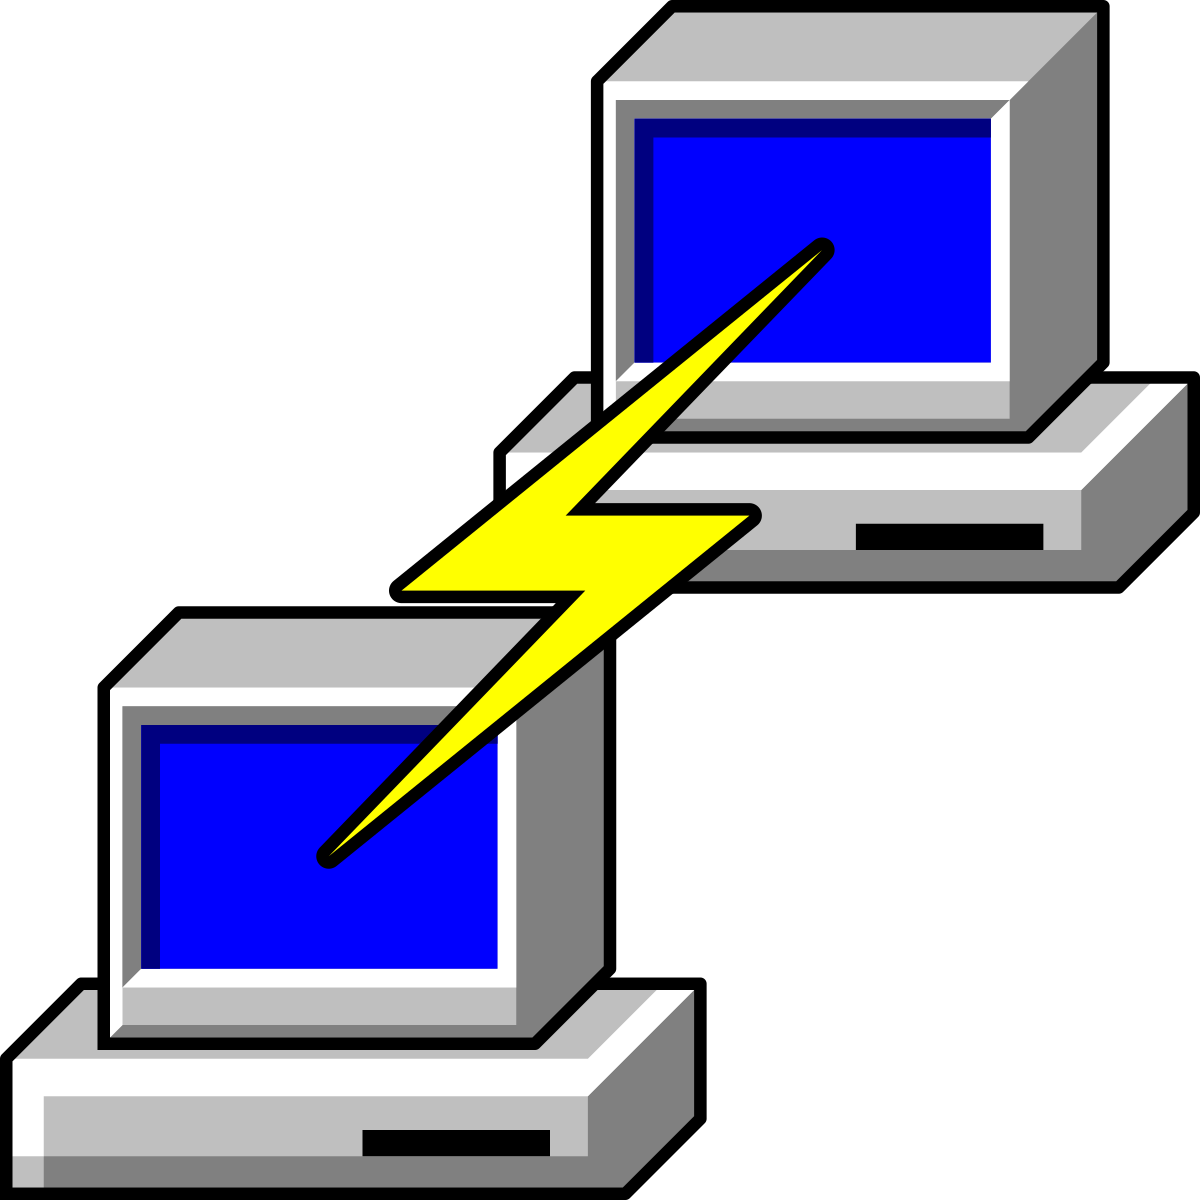
\includegraphics[width=3cm]{Images/Logo-Putty.png} & Putty & PuTTY est un logiciel client pour les protocoles de communication SSH, Telnet et Rlogin, permettant d'établir des connexions réseau sécurisées avec des ordinateurs distants. Il est utilisé principalement pour administrer des serveurs à distance, mais peut également être utilisé pour des transferts de fichiers et des sessions de console distantes. \\
\hline

\includegraphics[width=3cm]{Images/Logo-Raspberry.png} & Raspberry Pi Imager & Raspberry Pi Imager est un logiciel qui permet de facilement installer des systèmes d'exploitation sur une carte SD ou une clé USB pour Raspberry Pi. Il offre une interface graphique simple à utiliser pour sélectionner et télécharger les images d'OS disponibles. \\
\hline

\includegraphics[width=3cm]{Images/xminglogo.png} & Xming & Xming est un serveur d'affichage X open source qui permet d'exécuter des applications graphiques Linux sur des systèmes Windows. Il fournit un environnement graphique pour les applications Linux, ce qui permet aux utilisateurs de Windows d'accéder et d'interagir avec des applications Linux à distance. \\
\hline
\end{tabular}
\caption{Tableau du logiciel utilisées Partie 2 2}
\label{1}
\end{center}
\end{table}


\section{Présentation des locaux et Déploiement de Réseau MAN}
\subsection{Présentation des trois locaux}



\subsection{Définition du Réseau MAN}

Un réseau MAN est un type de réseau de communication qui couvre une zone géographique intermédiaire entre un réseau LAN et un réseau WAN. \cite{sze1985metropolitan} \\


\begin{figure}[H]
 \centering
    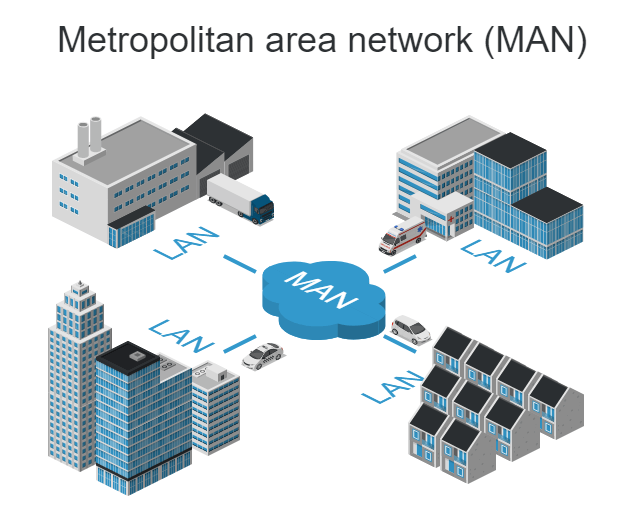
\includegraphics[width=15cm]{Images/network-man1.png}
    \caption{Metropolitan Area Network}
    \label{Chap2.3.1}
\end{figure}  
\smallskip

Contrairement à un réseau LAN qui est généralement limité à une seule installation ou à un seul site comme démontré dans la figure \ref{Chap2.3.1}, un réseau MAN s'étend sur une zone géographique plus étendue, comme une ville entière ou une zone métropolitaine.  \\


Dans le contexte de notre projet à Zeta Engineering, l'objectif est de relier les trois bureaux de l'entreprise situés à Rades Habib Bourgiba, Rades Meliane et Ezzahra via un réseau MAN pour permettre une communication efficace et une gestion centralisée des ressources.  \\


\subsection{Implémentation du MAN et le choix de TP-Link}

Pour établir notre réseau étendu (MAN), nous avons choisi d'utiliser le TP-Link CPE610. Ce point d'accès sans fil est spécialement conçu pour offrir une connectivité longue distance en utilisant la fréquence de 5 GHz. \\

Nous avons suivi les étapes d'assemblage et d'installation illustrées dans les images ci-dessous pour installer le TP-Link CPE610 : \\

\begin{figure}[H]
\centering
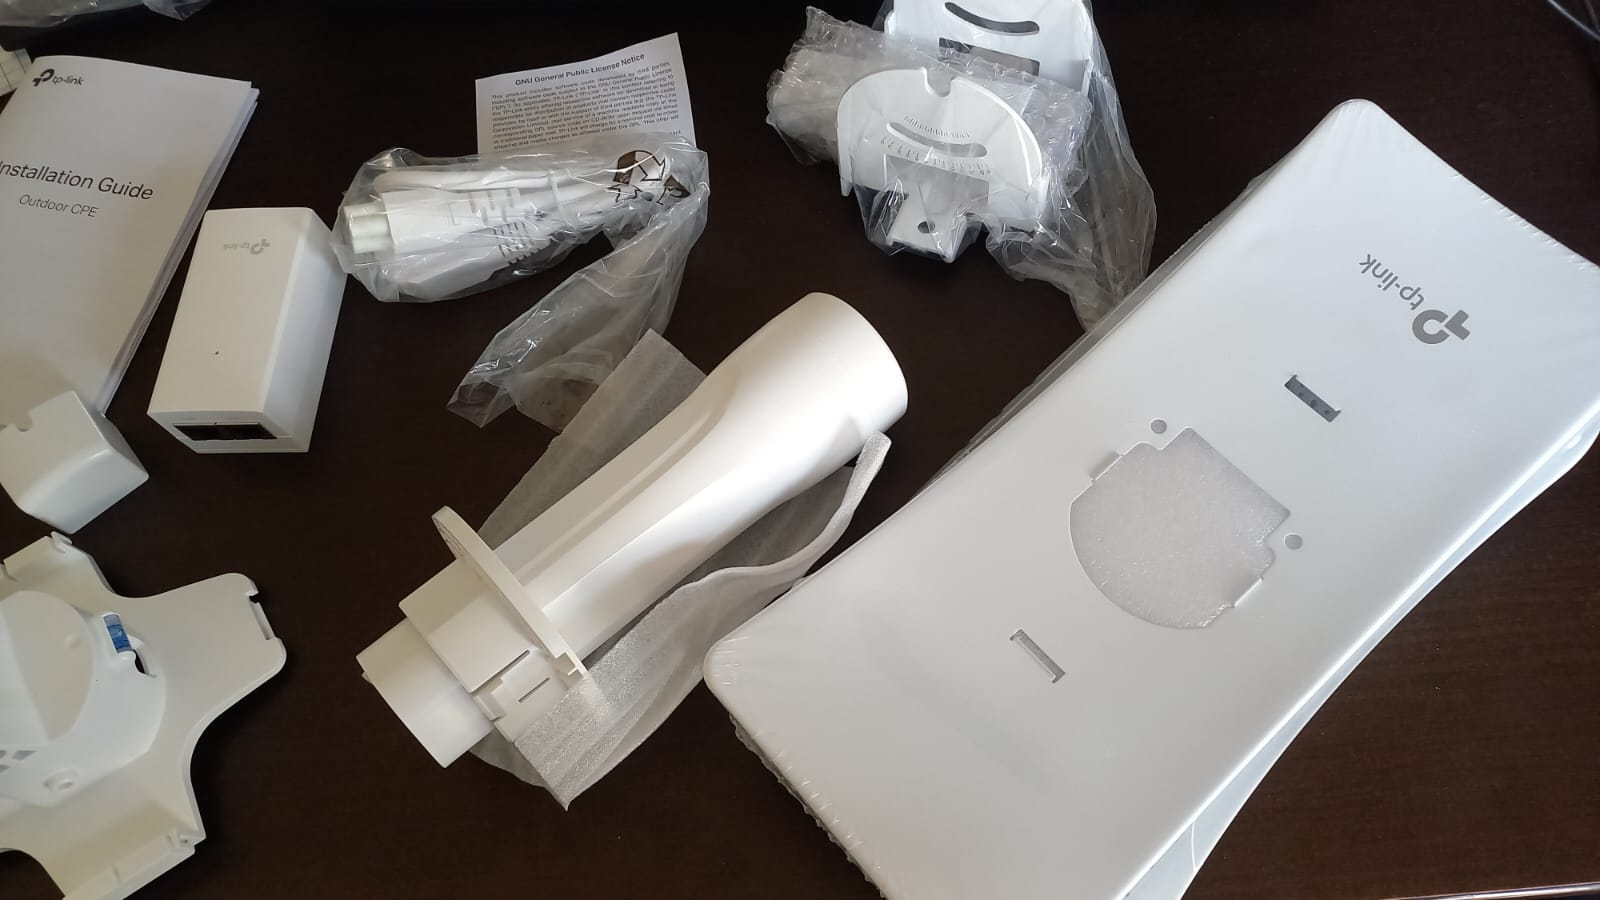
\includegraphics[width=15cm]{Images/SetupTPL4.jpg}
\caption{Déballage du TP-Link CPE610}
\label{Chap2.3.2}
\end{figure}

\begin{figure}[H]
\centering
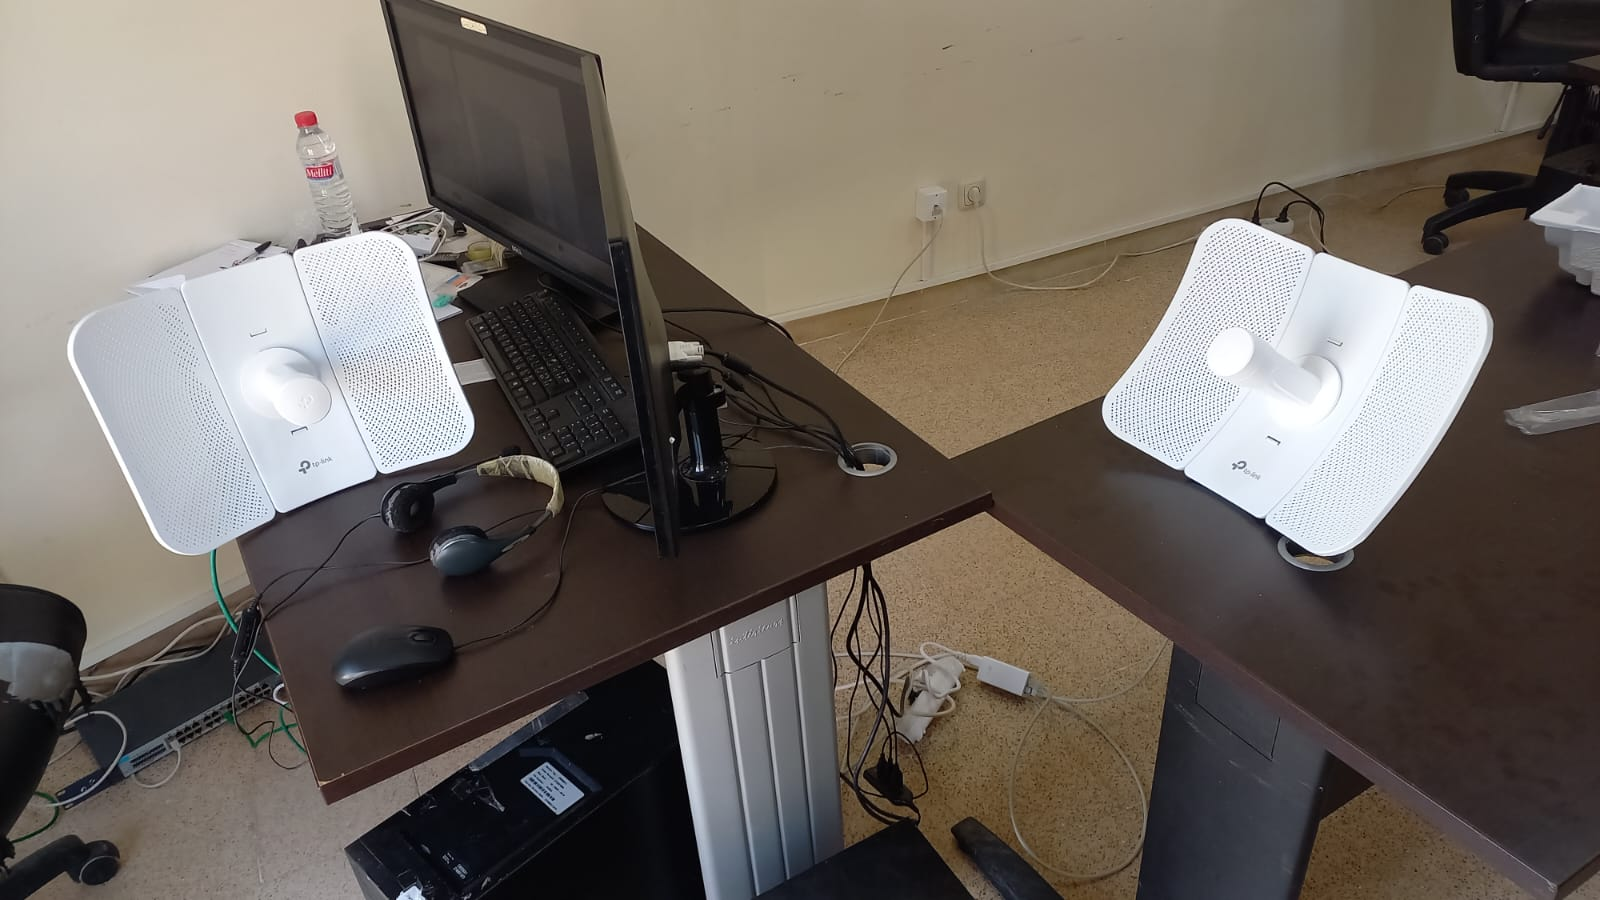
\includegraphics[width=15cm]{Images/SetupTPL1.jpg}
\caption{Assemblage des pièces du TP-Link CPE610}
\label{Chap2.3.4}
\end{figure}

Après avoir soigneusement assemblé les différentes composantes du TP-Link, nous sommes en mesure d'accéder à son panneau d'administration via une connexion LAN. À partir de là, nous entamons le processus d'initialisation et de configuration.

La Figure \ref{Chap2.3.5} illustre l'étape d'initialisation du TP-Link, où nous configurons les paramètres essentiels pour son bon fonctionnement.

\begin{figure}[H]
\centering
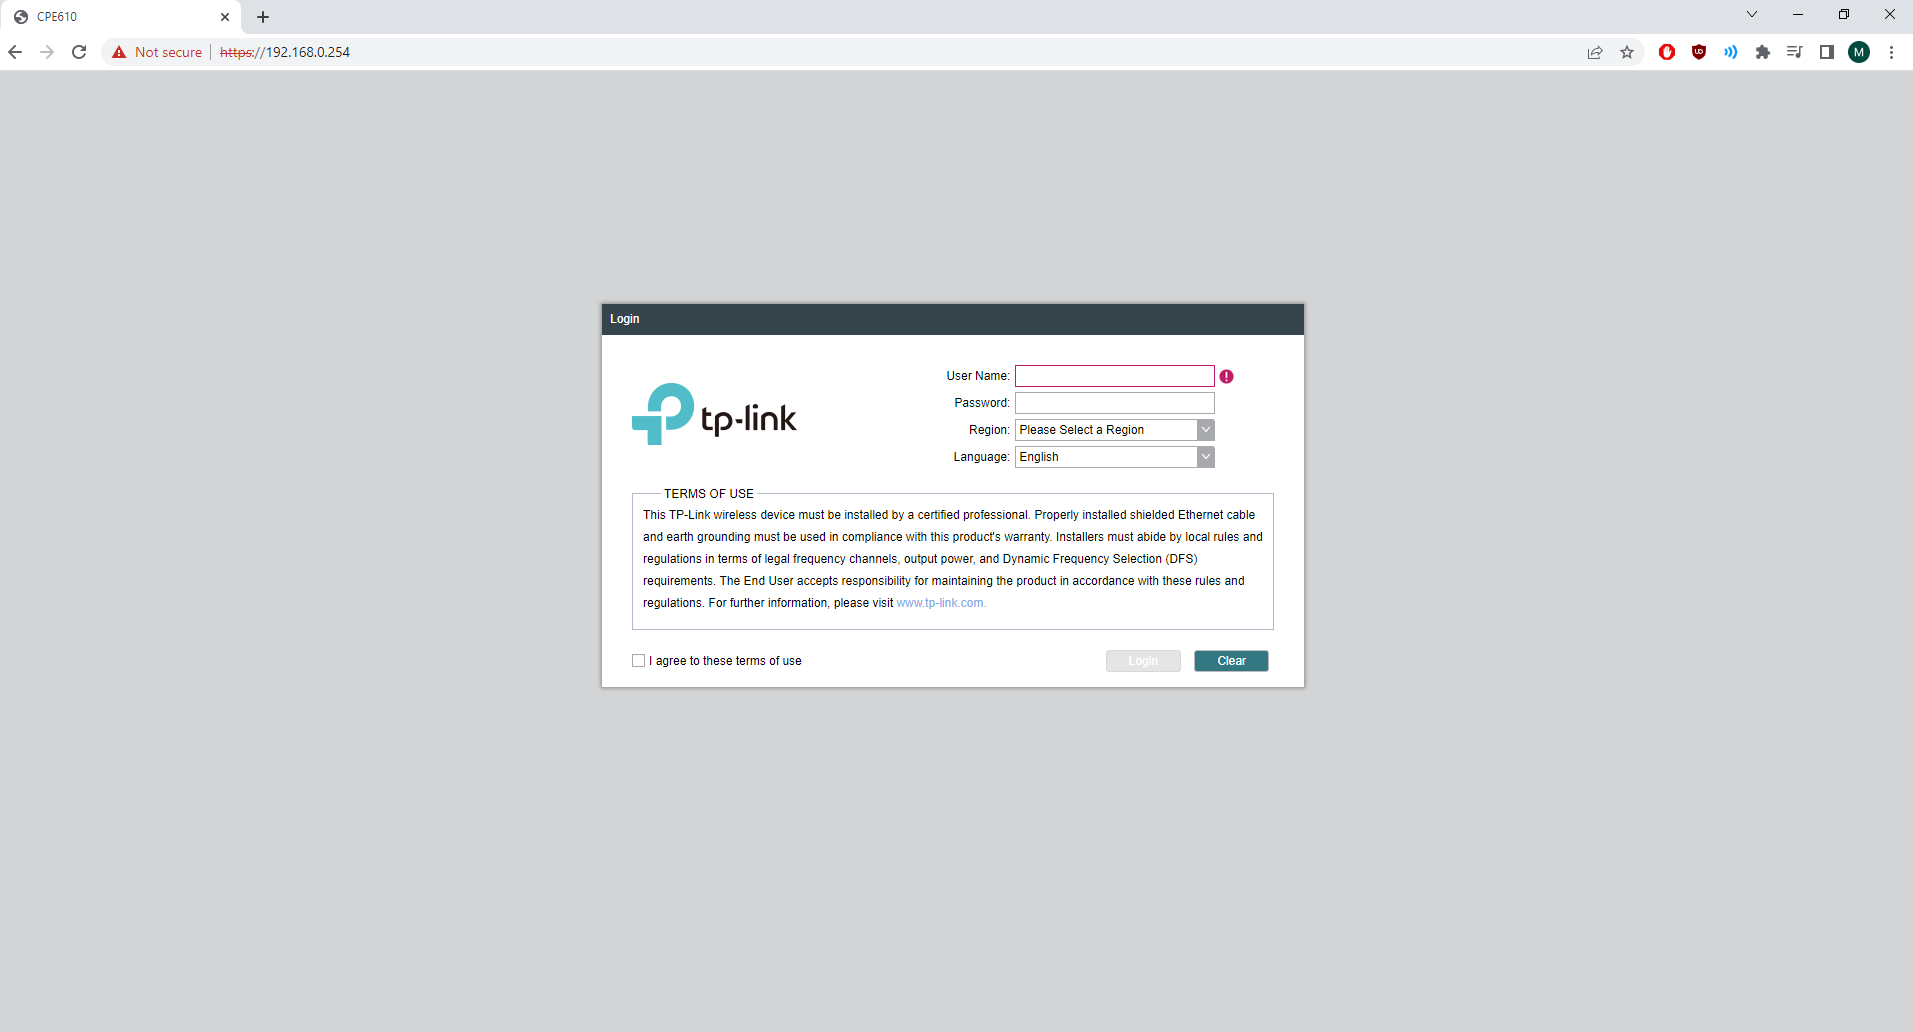
\includegraphics[width=15cm]{Images/tplink3.png}
\caption{Initialisation du TP-Link}
\label{Chap2.3.5}
\end{figure}

La configuration en mode test est représentée dans la Figure \ref{Chap2.3.6}, nous permettant de vérifier les performances du dispositif avant une utilisation complète.

\begin{figure}[H]
\centering
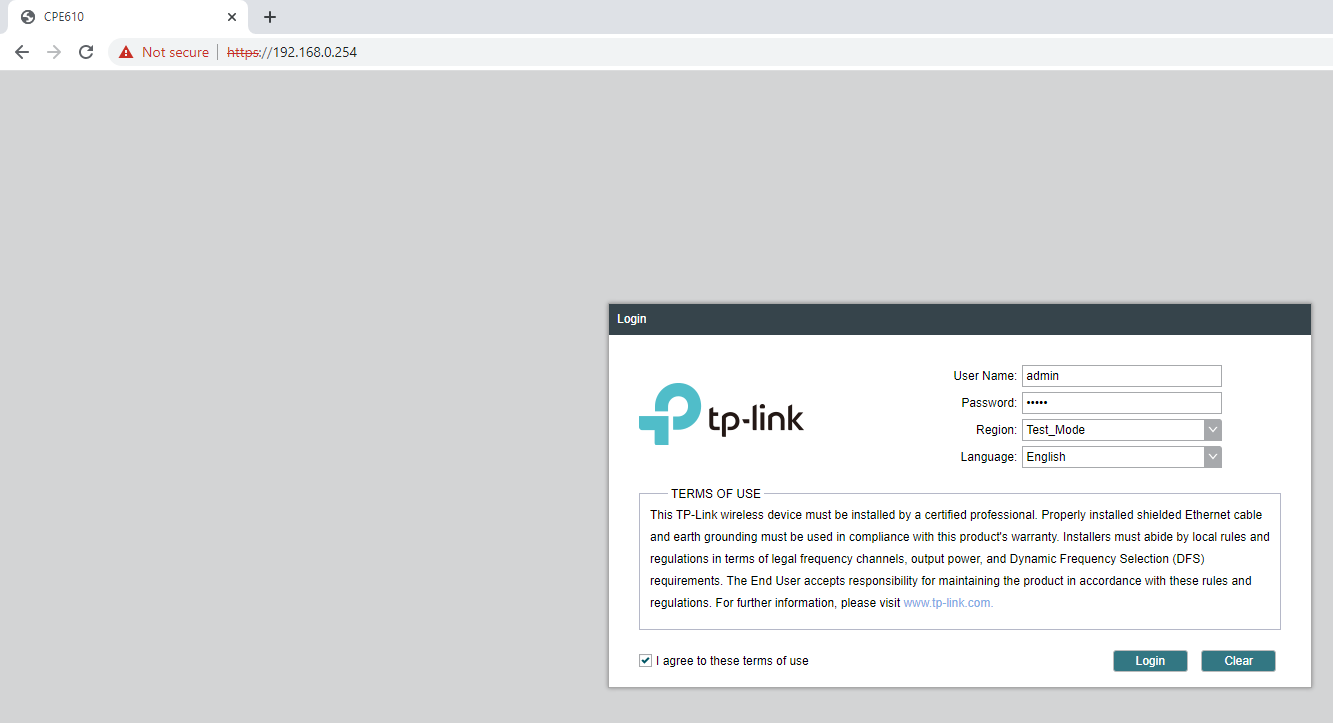
\includegraphics[width=15cm]{Images/tplink33.png}
\caption{Initialisation du TP-Link en mode test}
\label{Chap2.3.6}
\end{figure}

Le panneau de contrôle complet du TP-Link est dépeint dans la Figure \ref{Chap2.3.7}, où nous pouvons régler et surveiller divers paramètres pour garantir un réseau stable.

\begin{figure}[H]
\centering
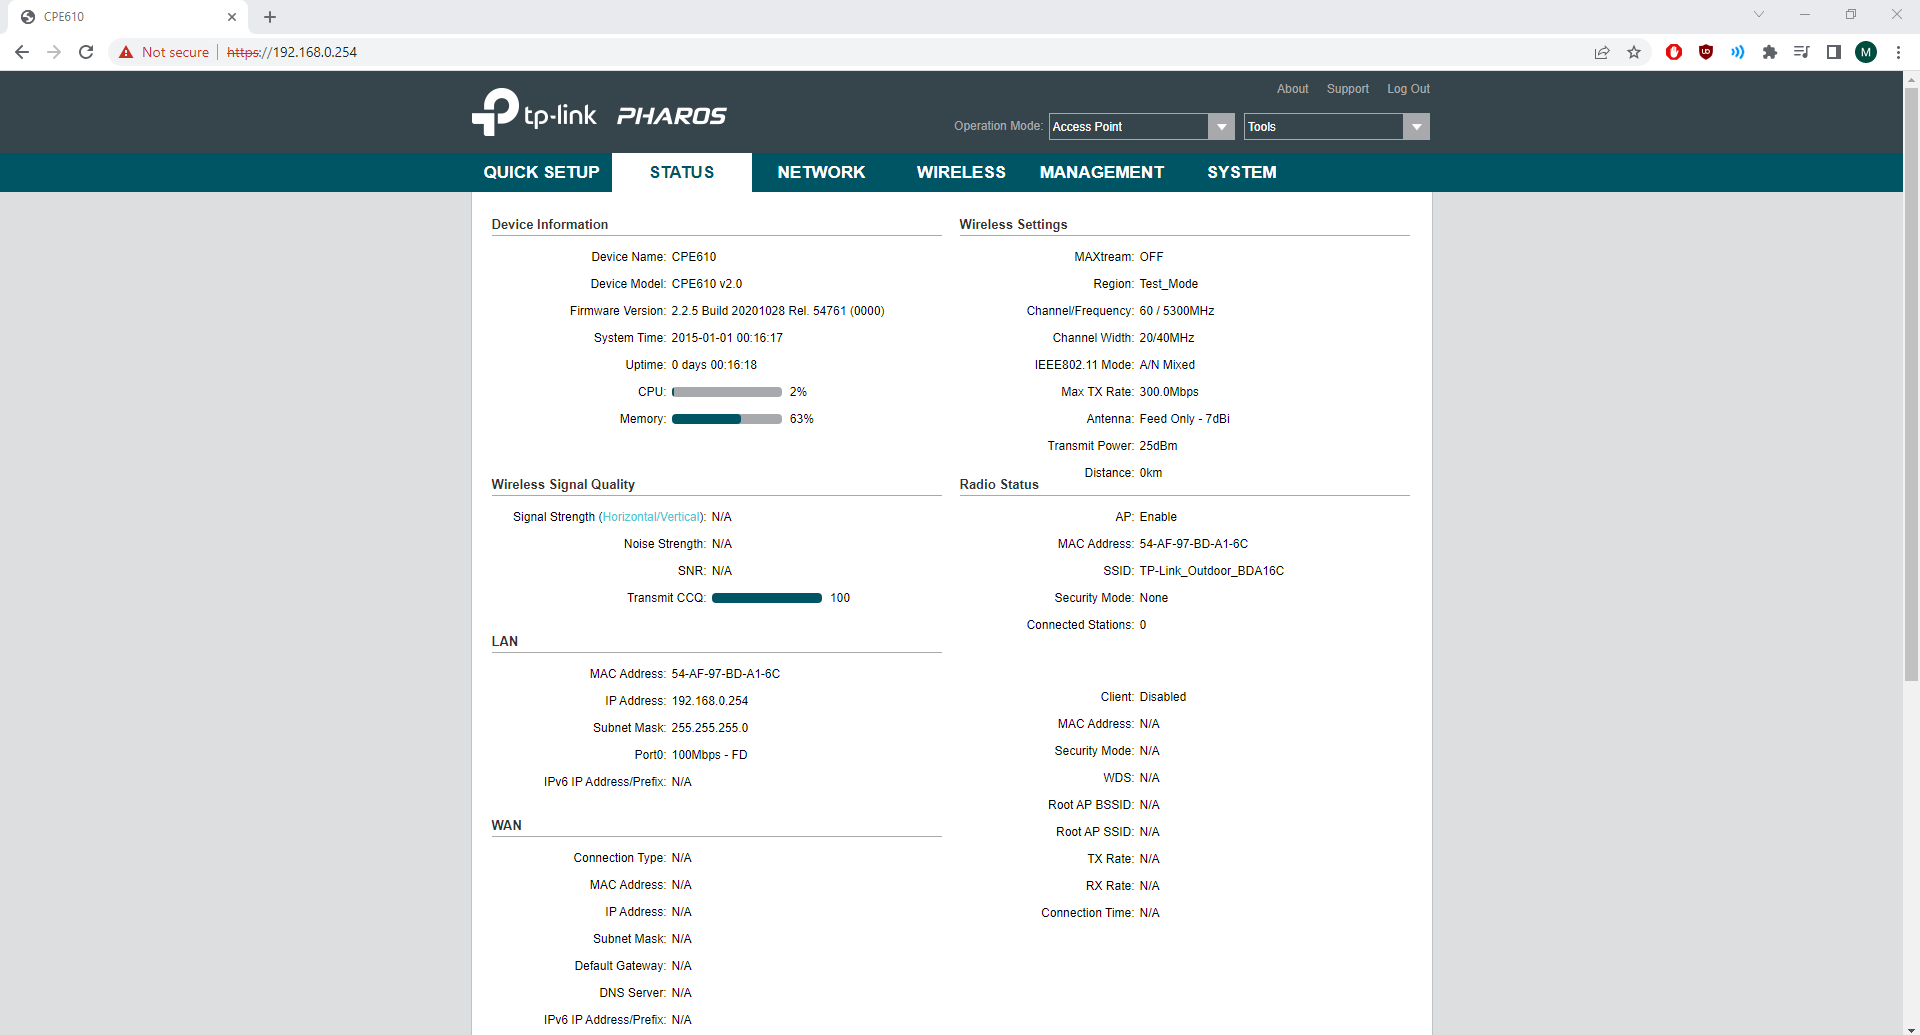
\includegraphics[width=15cm]{Images/tplink34.png}
\caption{Panneau de contrôle du TP-Link}
\label{Chap2.3.7}
\end{figure}

Les Figures \ref{Chap2.3.8} et \ref{Chap2.3.9} montrent respectivement les étapes d'initialisation de l'émetteur et du récepteur du TP-Link, éléments clés pour établir une connexion fiable.

\begin{figure}[H]
\centering
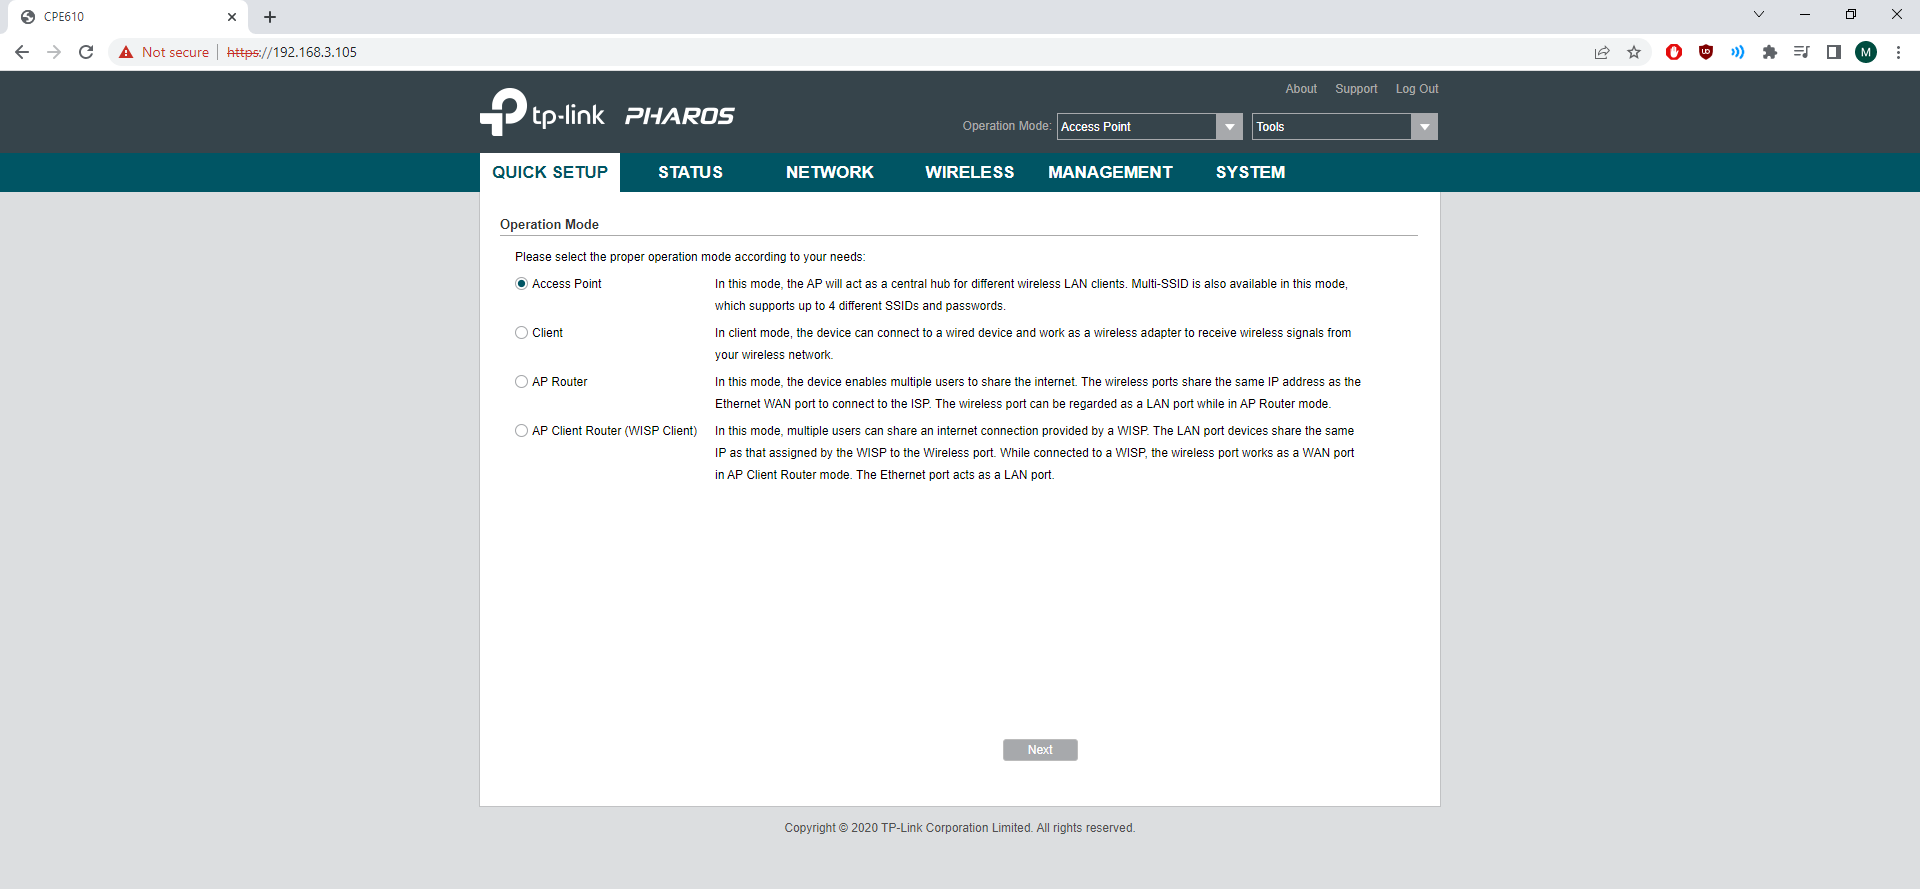
\includegraphics[width=15cm]{Images/tplink35.png}
\caption{Initialisation de l'émetteur}
\label{Chap2.3.8}
\end{figure}

\begin{figure}[H]
\centering
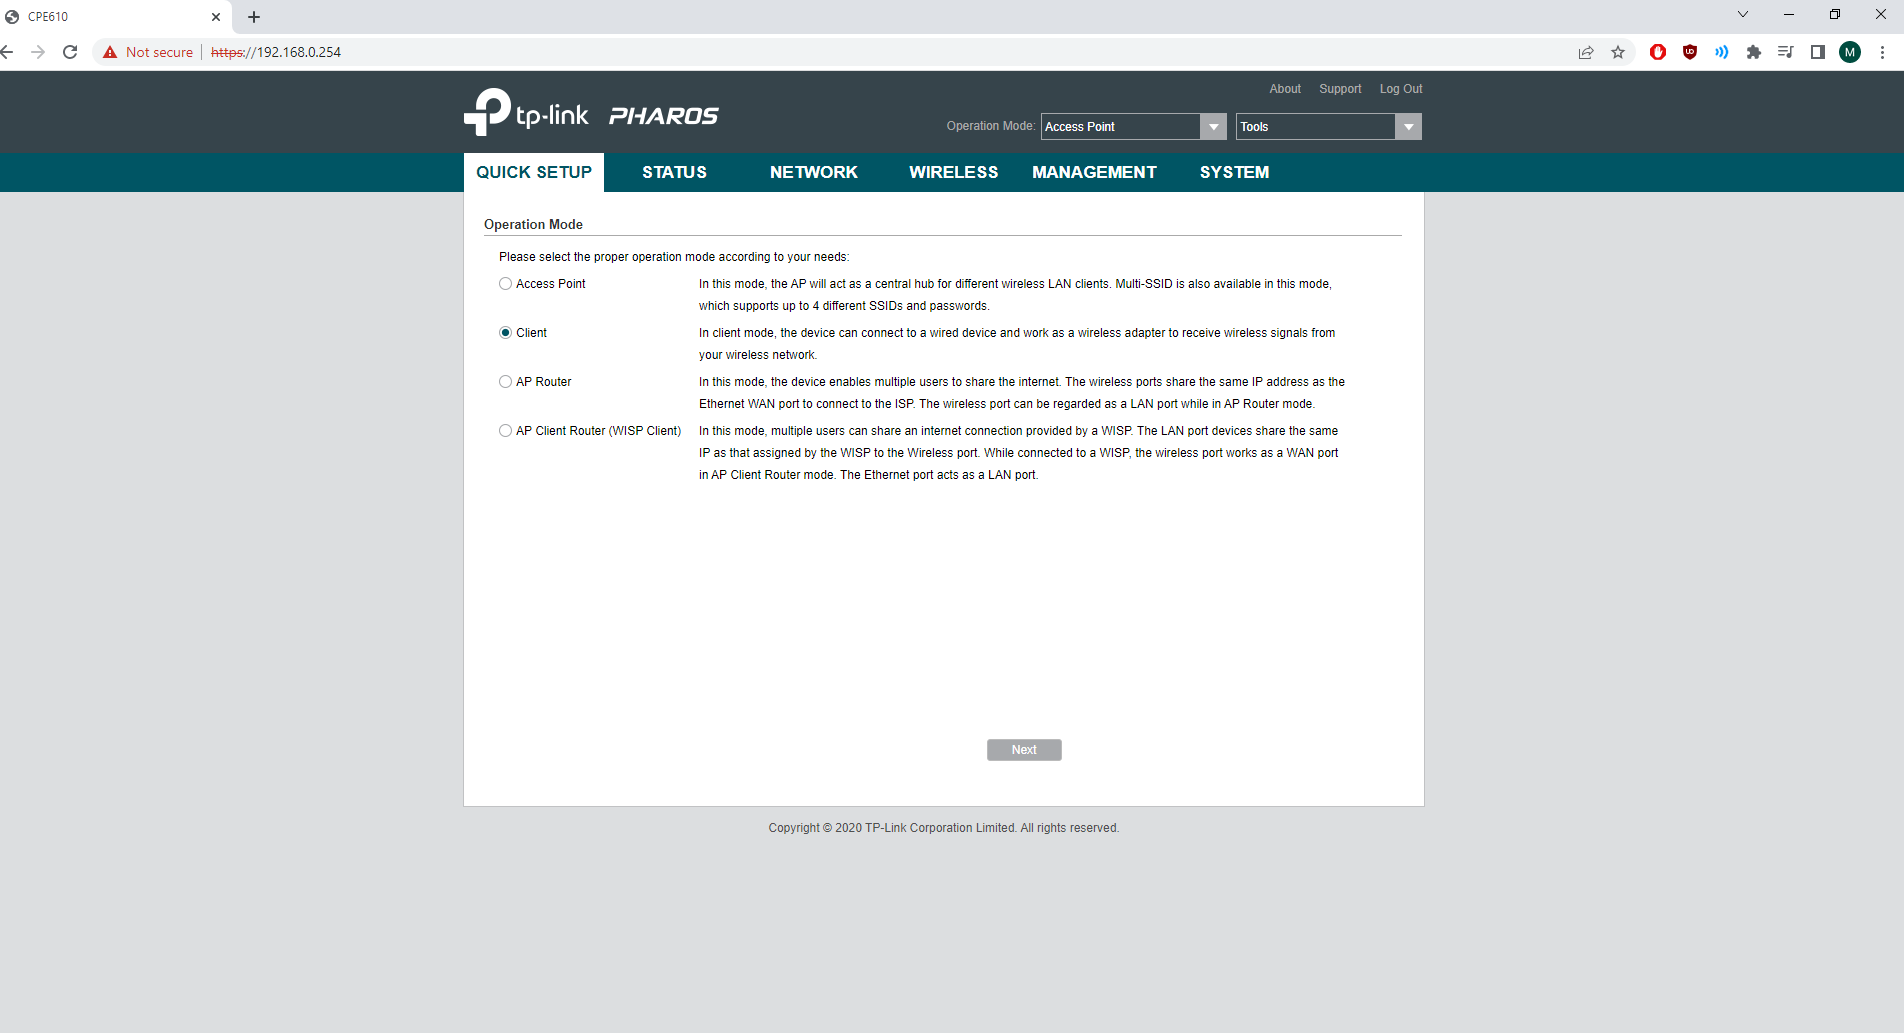
\includegraphics[width=15cm]{Images/tplink36.png}
\caption{Initialisation du récepteur}
\label{Chap2.3.9}
\end{figure}

Les étapes finales de vérification de la connexion entre le point d'accès TP-Link et le client TP-Link sont détaillées dans les Figures \ref{Chap2.3.10} et \ref{Chap2.3.11}.

\begin{figure}[H]
\centering
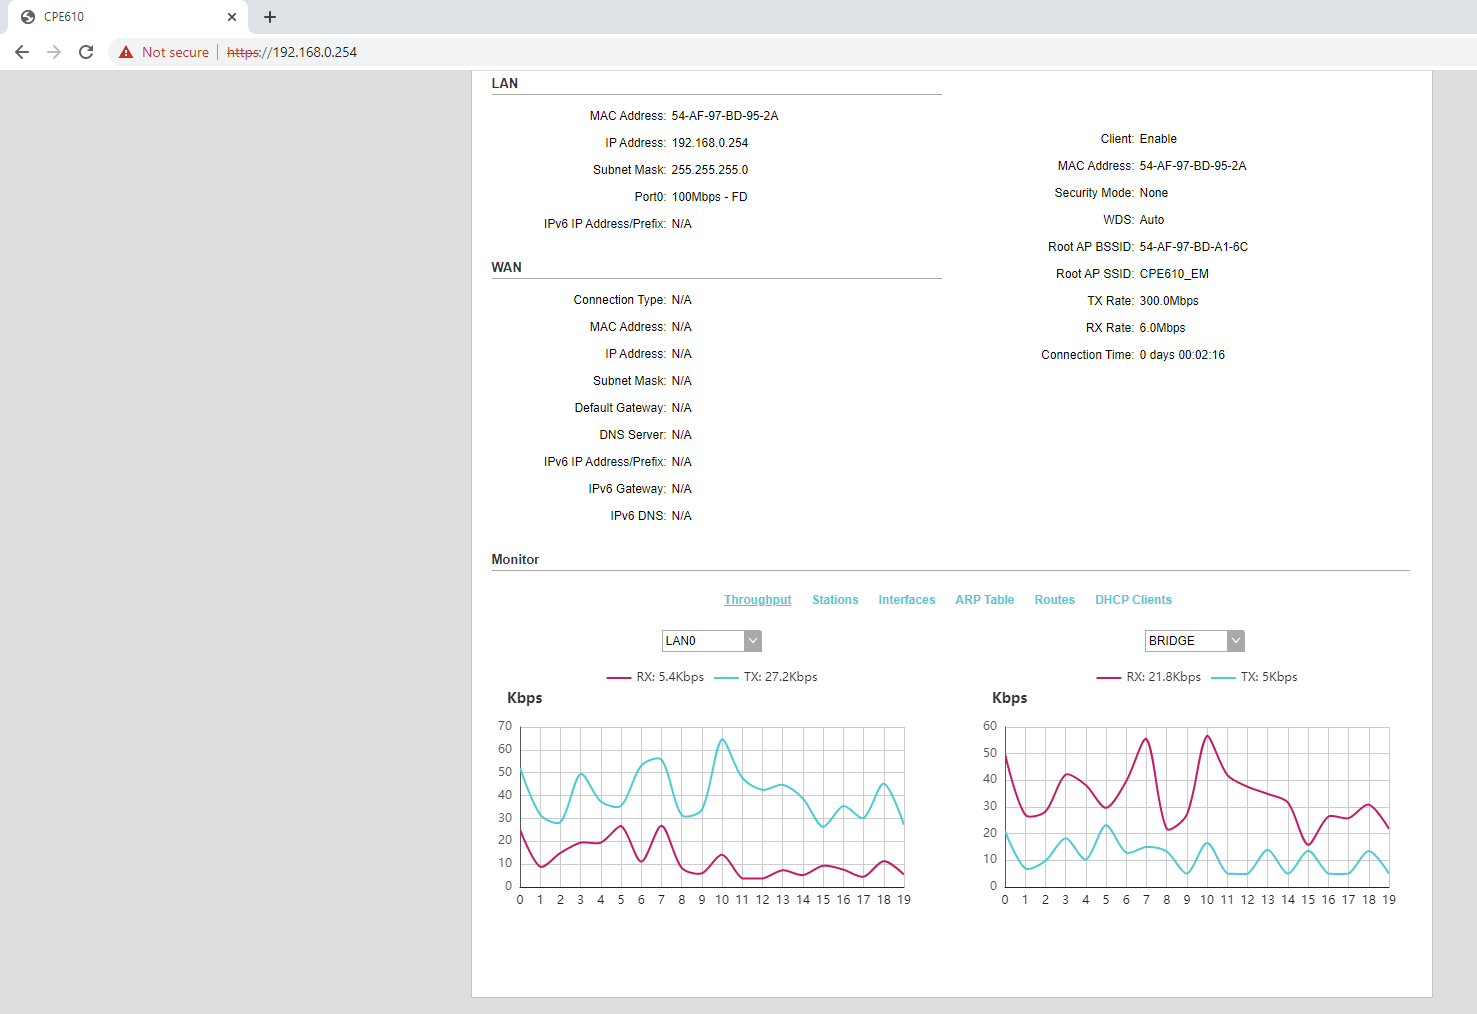
\includegraphics[width=15cm]{Images/tplink37.png}
\caption{Test de connexion entre le point d'accès TP-Link et le client TP-Link}
\label{Chap2.3.10}
\end{figure}

\begin{figure}[H]
\centering
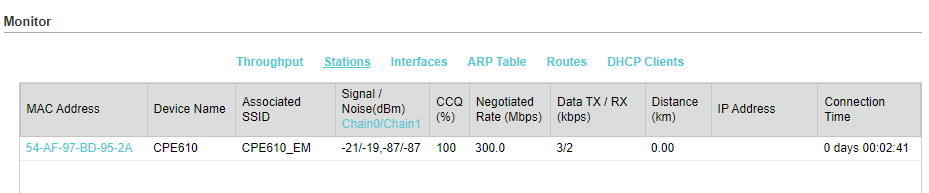
\includegraphics[width=15cm]{Images/TPLink4.png}
\caption{Test de connexion entre le point d'accès TP-Link et le client TP-Link}
\label{Chap2.3.11}
\end{figure}

Enfin, la Figure \ref{Chap2.3.12} met en évidence l'installation réussie du TP-Link CPE610 à Rades Melian, marquant une étape cruciale de notre déploiement.

\begin{figure}[H]
\centering
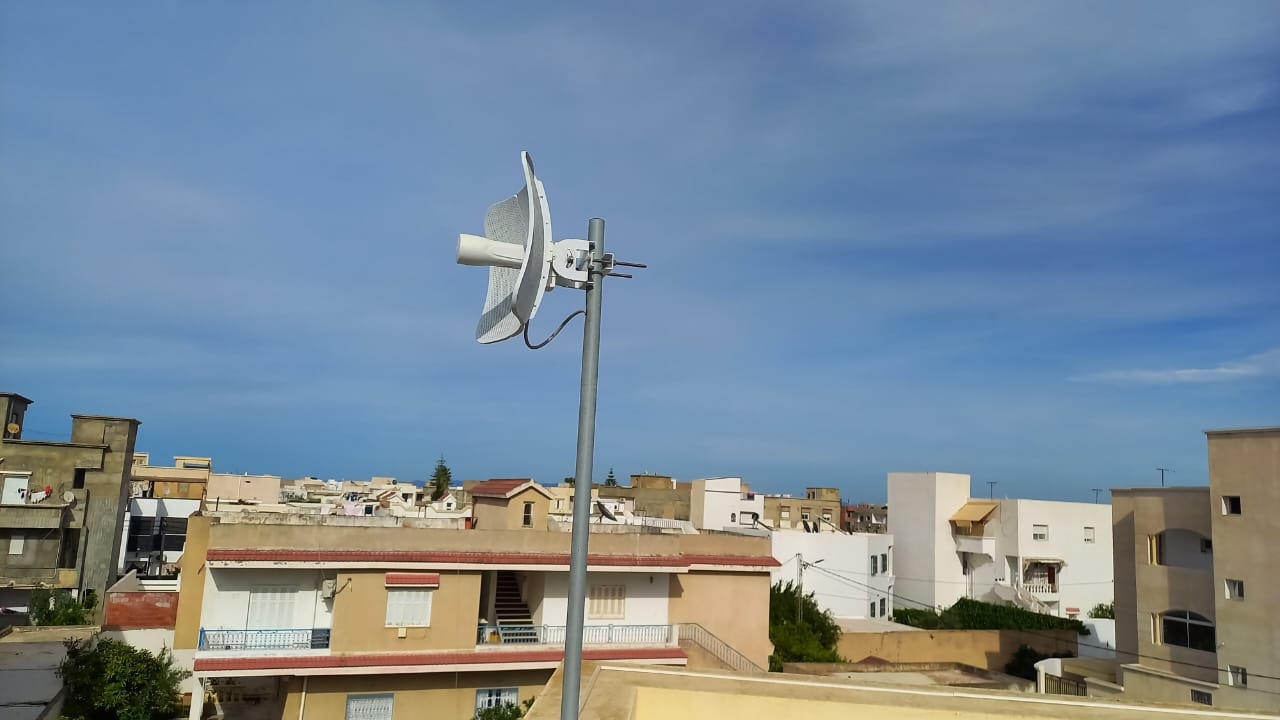
\includegraphics[width=15cm]{Images/BRadesMelian-TPLinkCEP610-1.jpeg}
\caption{Installation du TP-Link CPE610 à Rades Melian}
\label{Chap2.3.12}
\end{figure}

En suivant ces étapes, nous avons réussi à tester nos TP-Link et nous allons maintenant procéder à leur installation dans les différents bureaux. \\

\section{L'architecture Réseau Rades}

Dans cette section nous présentons la topologie en GNS3 puis sa configuration et implémentation en Rades.

\subsection{Topologie en GNS3}

Dans cette section, nous allons présenter l'architecture réseau de l'office de Rades. \\

\begin{figure}[H]
 \centering
    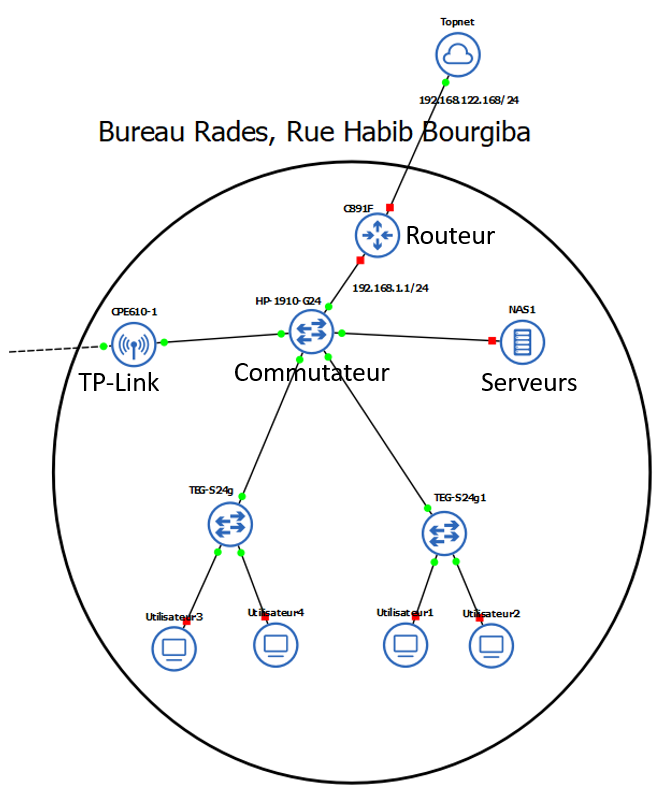
\includegraphics[width=16cm]{Images/BRades-Topologie.png}
    \caption{Topologie du réseau de l'Office de Rades}
    \label{Chap2.2.0}
\end{figure}




L'objectif principal de cette simulation est de démontrer l'efficacité de l'architecture réseau de l'office de Rades. Nous avons modélisé les différents équipements du réseau dans la figure \ref{Chap2.2.0}, tel que le routeur C891F qui distribue l'Internet reçu de Topnet vers le commutateur principale HP-1910-G24 et d'après cette commutateur nous distribuons l'accés a l'internet vers les utilsateurs et les lié avec les serveurs disponible de la société.

Cette simulation nous a permis de mettre en évidence la performance et la fiabilité de notre architecture réseau. Nous avons également pu identifier et résoudre les problèmes potentiels avant leur apparition dans le réseau réel, en modifiant les paramètres de configuration ou en ajoutant de nouveaux équipements si nécessaire. \\

La visualisation de la topologie réseau dans GNS3 est un outil très utile pour la planification et la gestion du réseau, ainsi que pour la formation du personnel technique. \\



\subsection{Configuration en GNS3}

Dans cette section, nous présentons la configuration de notre réseau en utilisant GNS3. Tout d'abord, nous montons la topologie du réseau dans la figure \ref{Chap2.2.1}, où nous avons accès à la console du routeur. 


\begin{figure}[H]
 \centering
    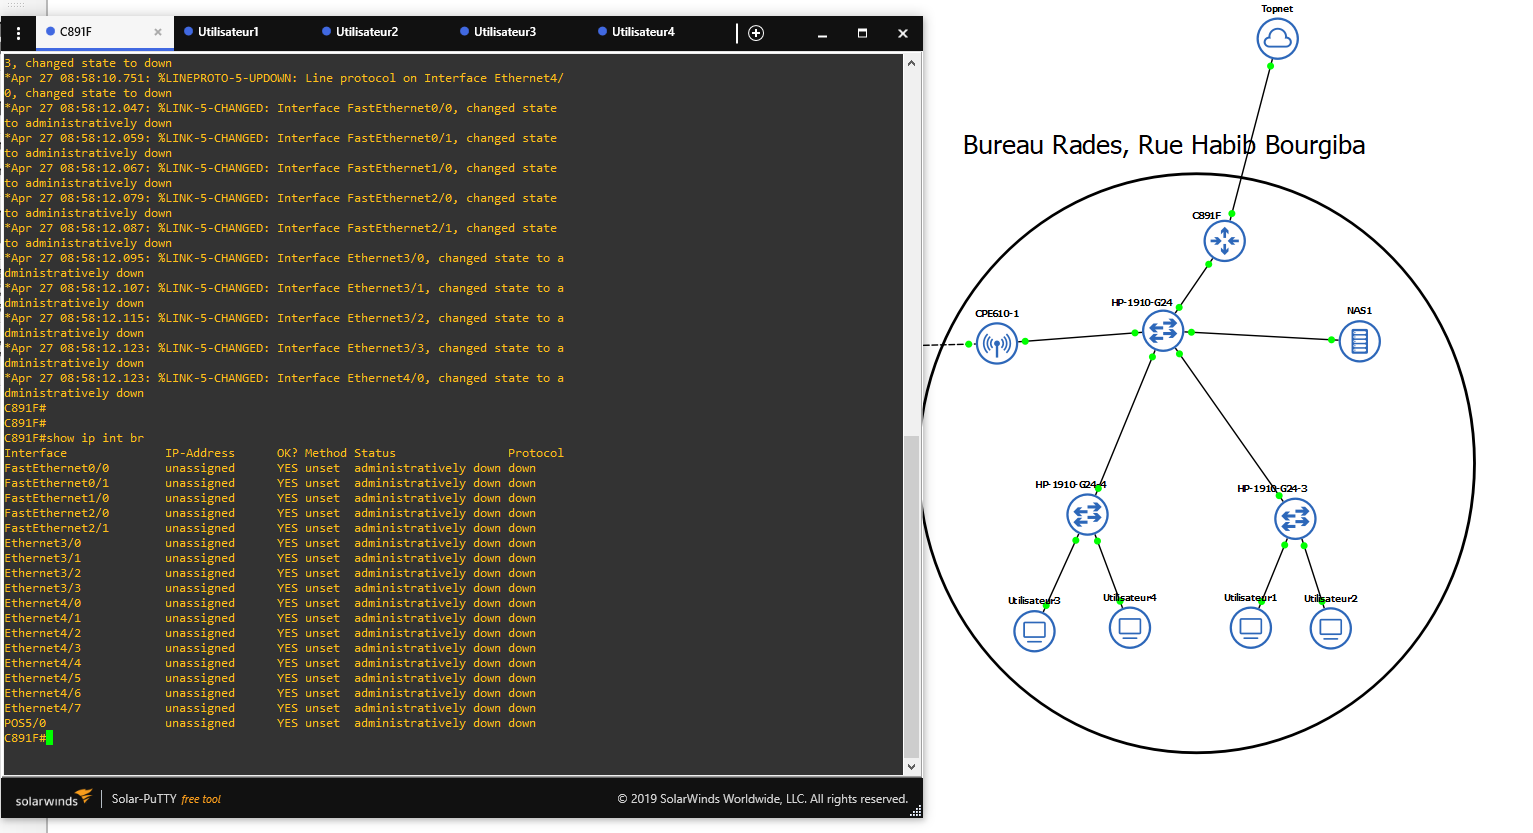
\includegraphics[width=16cm]{Images/BRades-Topologie1.png}
    \caption{Topologie du réseau de l'Office de Rades 2}
    \label{Chap2.2.1}
\end{figure}


Ensuite, dans la figure \ref{Chap2.2.2}, nous avons obtenu une adresse IP DHCP pour notre console et activé l'option "domain-lookup".  \\


\bigskip
\bigskip
\bigskip
\bigskip


\begin{figure}[H]
 \centering
    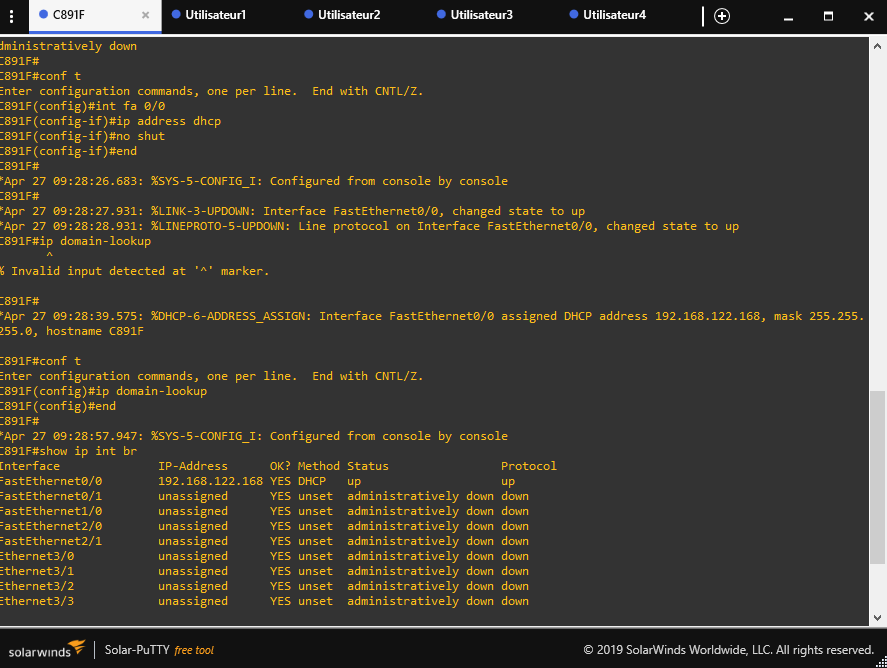
\includegraphics[width=16cm]{Images/BRades-Topologie2.png}
    \caption{Réglage de l'IP adresse}
    \label{Chap2.2.2}
\end{figure}

\smallskip


Dans la figure \ref{Chap2.2.3}, nous effectuons un ping réussi vers "8.8.8.8", ce qui indique que nous avons accès à l'Internet, et également vers "www.google.com" grâce à l'option "domain-lookup" que nous avons utilisée. \\

\bigskip
\bigskip
\bigskip
\bigskip

\begin{figure}[H]
 \centering
    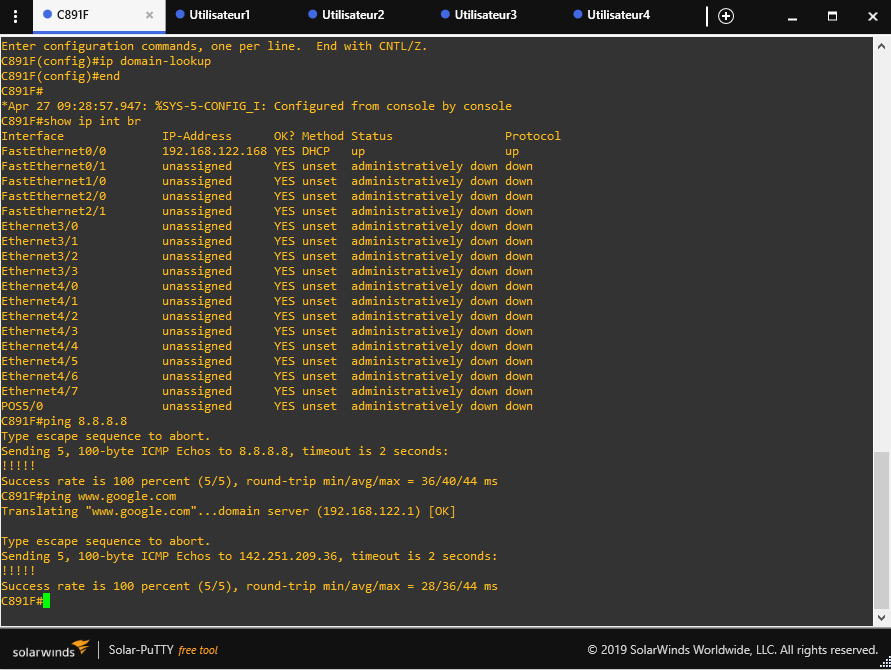
\includegraphics[width=16cm]{Images/BRades-Topologie3.png}
    \caption{Test de connexion}
    \label{Chap2.2.3}
\end{figure}

Dans la figure \ref{Chap2.2.4}, nous ajoutons un réseau interne "192.168.1.1/24".  \\

\begin{figure}[H]
 \centering
    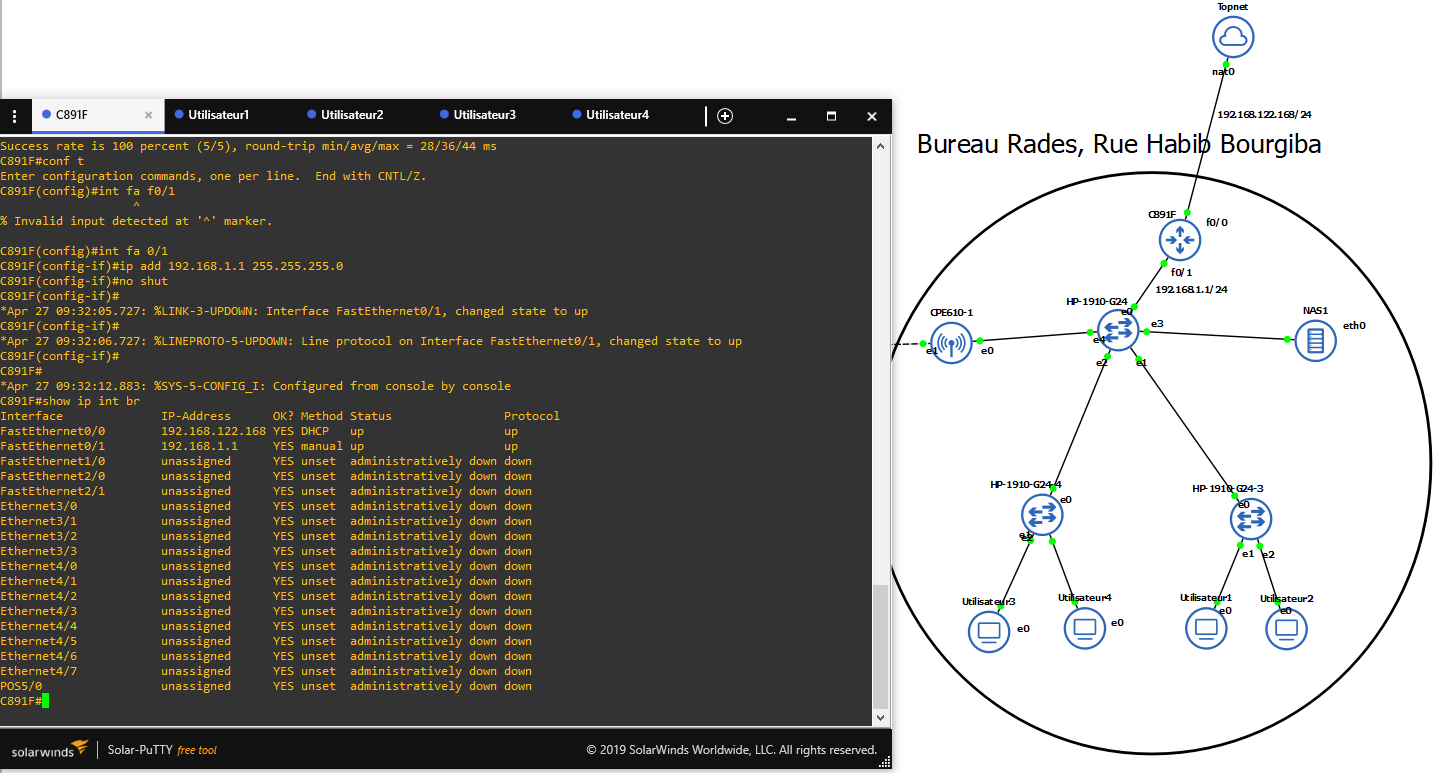
\includegraphics[width=16cm]{Images/BRades-Topologie4.png}
    \caption{Configurer le Port f0/1}
    \label{Chap2.2.4}
\end{figure}

Cependant, nous constatons dans la figure \ref{Chap2.2.5} que nous ne pouvions pas toujours accéder à internet depuis la machine de la société. \\

\begin{figure}[H]
 \centering
    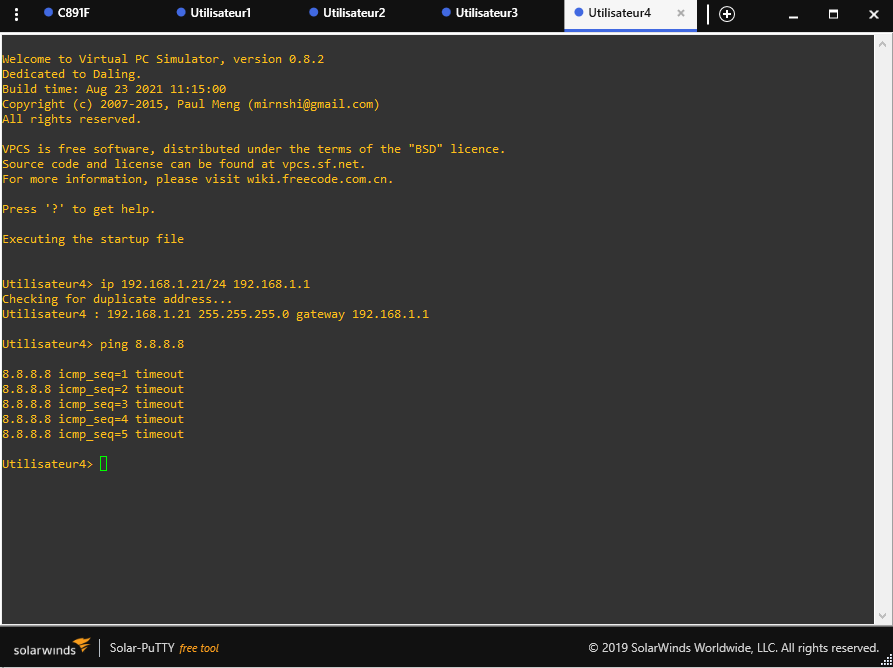
\includegraphics[width=16cm]{Images/BRades-Topologie5.png}
    \caption{Ping de Utilisateur4 vers l'internet}
    \label{Chap2.2.5}
\end{figure}

\smallskip


Dans la figure \ref{Chap2.2.6}, nous observons que toutes les machines ont accès à Internet et peuvent communiquer entre elles au sein du réseau local.



\smallskip

\begin{figure}[H]
 \centering
    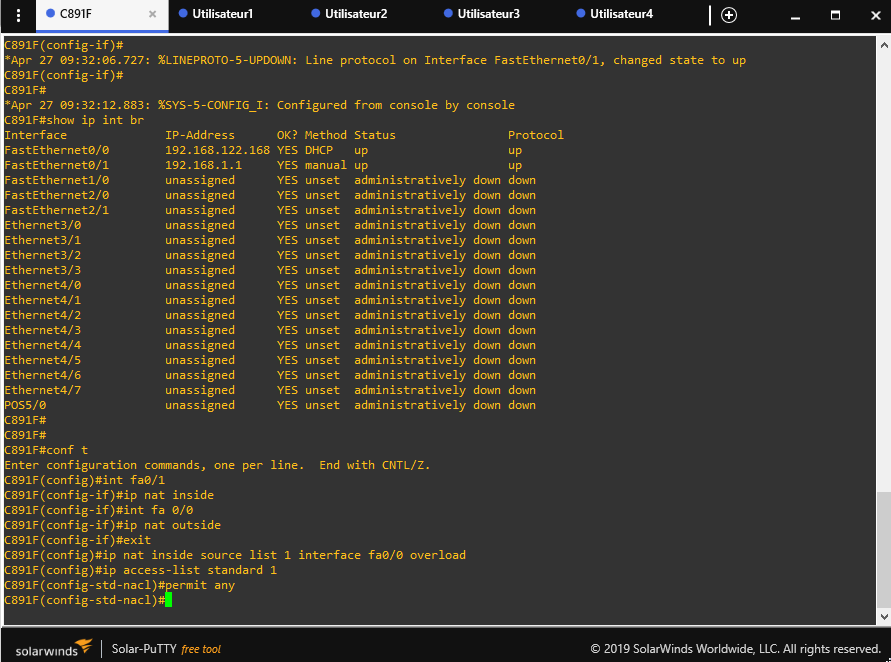
\includegraphics[width=16cm]{Images/BRades-Topologie6.png}
    \caption{Configuration de Routeur}
    \label{Chap2.2.6}
\end{figure}

\smallskip



Dans les figures \ref{Chap2.2.7}, \ref{Chap2.2.8} et \ref{Chap2.2.9}, nous constatons que toutes les machines avaient accès à internet et pouvaient communiquer entre elles dans le réseau local. \\

\smallskip

\begin{figure}[H]
 \centering
    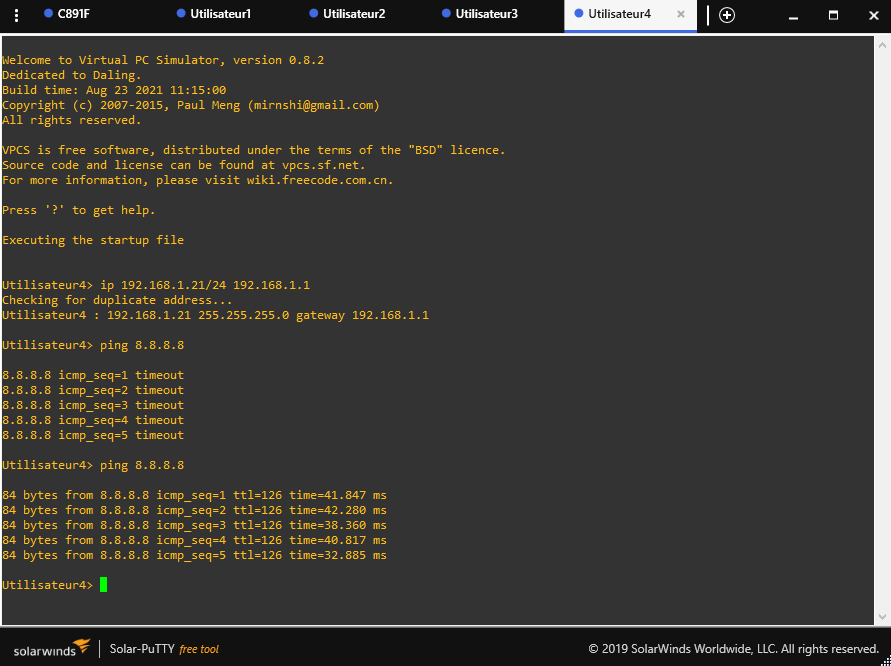
\includegraphics[width=16cm]{Images/BRades-Topologie7.png}
    \caption{Test de connexion des utilisateurs}
    \label{Chap2.2.7}
\end{figure}

\smallskip

\begin{figure}[H]
 \centering
    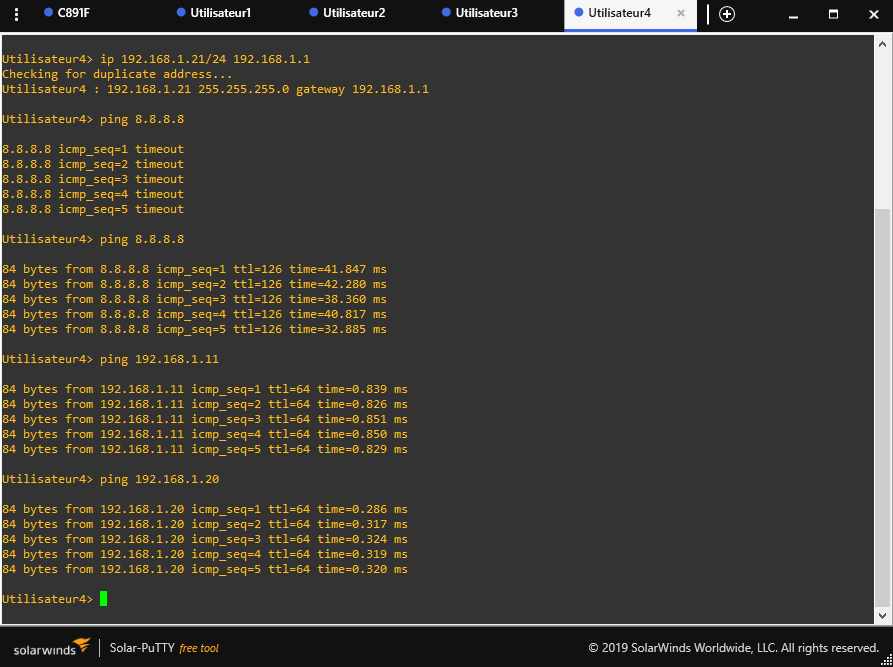
\includegraphics[width=16cm]{Images/BRades-Topologie8.png}
    \caption{Test de connexion des utilisateurs 2}
    \label{Chap2.2.8}
\end{figure}

\smallskip

\begin{figure}[H]
 \centering
    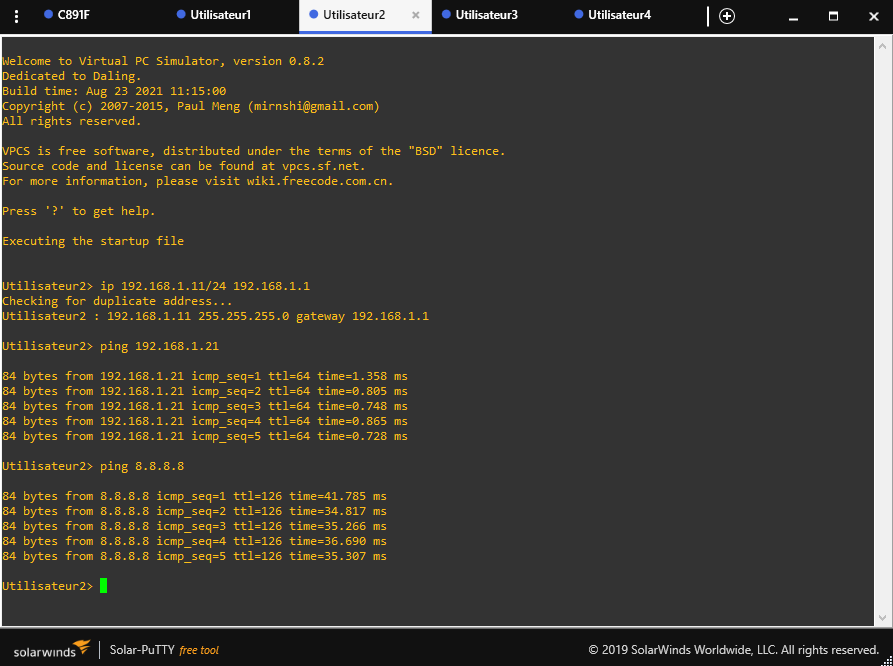
\includegraphics[width=16cm]{Images/BRades-Topologie9.png}
    \caption{Test de connexion des utilisateurs 3}
    \label{Chap2.2.9}
\end{figure}

\smallskip

En résumé, nous avons configuré notre réseau en utilisant GNS3 en étapes, en veillant à ce que toutes les machines aient accès à internet et puissent communiquer entre elles dans le réseau local. \\


  
\subsection{Implémentation}

Étant donné que l'infrastructure de fibre optique de Topnet/Telecom n'est pas disponible à proximité du bureau central de Rades Melian, nous trouvons une solution en achetant une connexion Internet par fibre optique dans deux autres bureaux, Rades (20 Mbps) et Ezzahara (100 Mbps), et en les reliant via un réseau MAN (Metropolitan Area Network). Les deux connexions sont connectées à un routeur Cisco 891F configuré par l'équipe de Topnet, qui distribue le réseau vers un commutateur Cisco v19-10 24G. Le routeur Cisco 891F est représenté dans la Figure \ref{Chap2.2.10}.

\begin{figure}[H]
\centering
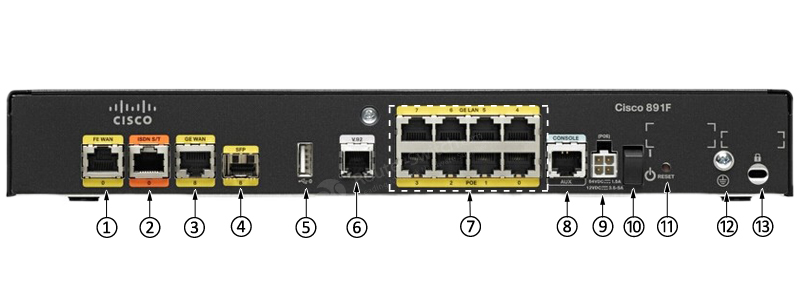
\includegraphics[width=15cm]{Images/C891F_1.jpg}
\caption{Routeur Cisco 891F}
\label{Chap2.2.10}
\end{figure}

À partir du commutateur, nous pouvons accéder à d'autres commutateurs qui permettent la connectivité des PC et des objets connectés dans le bureau. La Figure \ref{Chap2.2.11} montre l'interconnexion des commutateurs pour le bureau de Rades.

\begin{figure}[H]
\centering
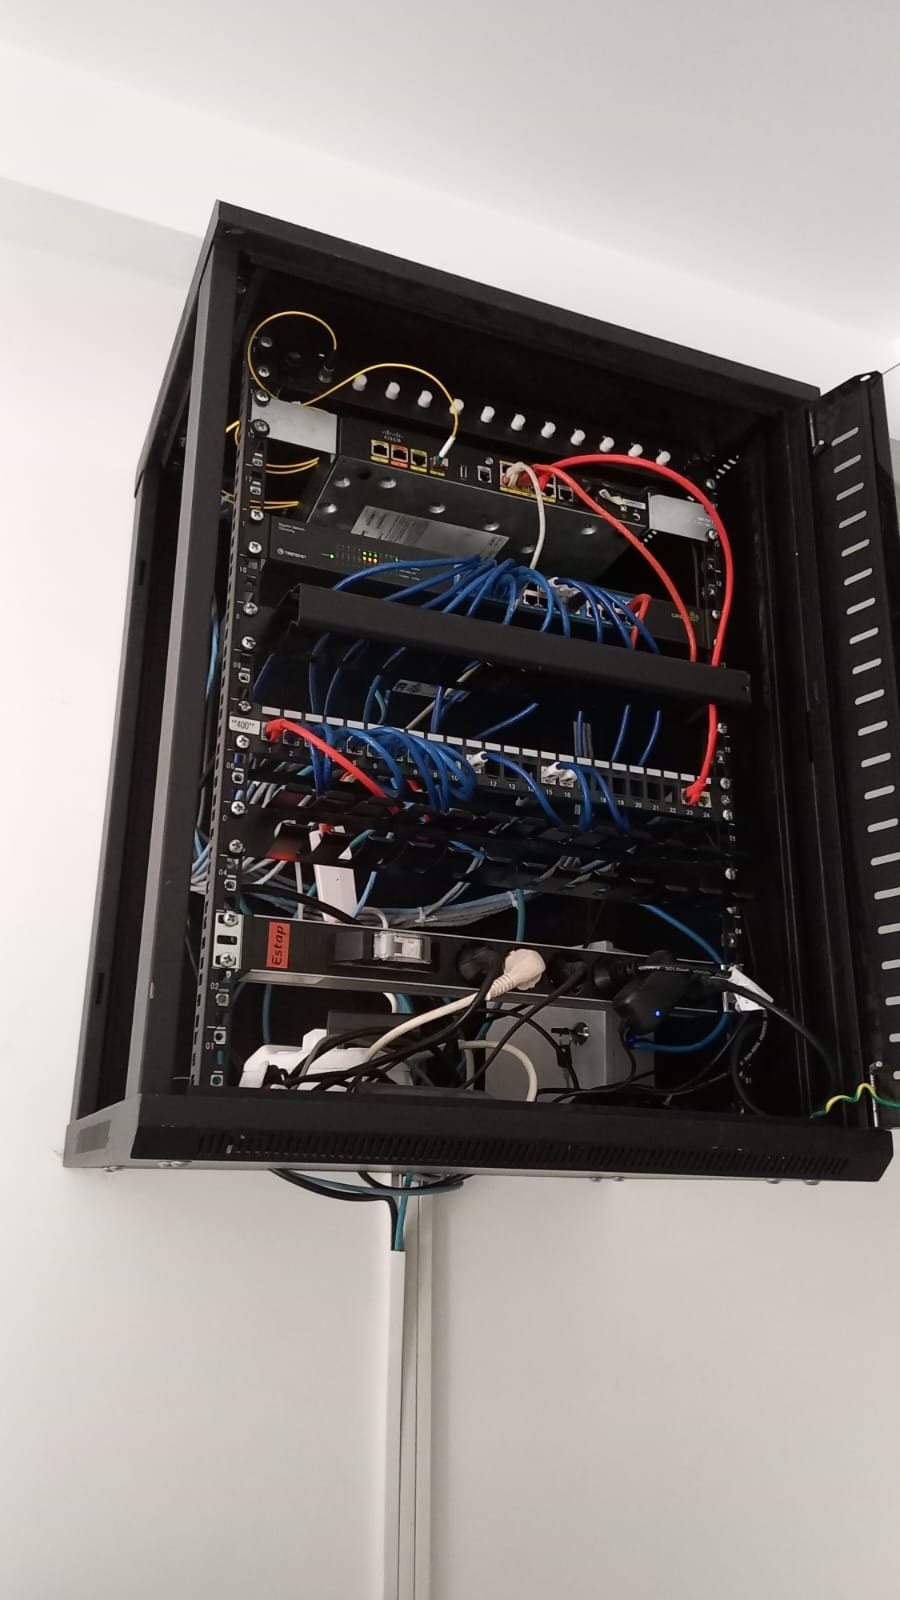
\includegraphics[width=7cm,height=12cm]{Images/BRades-ArmoirePrincipal.jpg}
\caption{Interconnexion des commutateurs pour le bureau de Rades}
\label{Chap2.2.11}
\end{figure}

\section{L'architecture Réseau Rades Mélian}

Dans cette section nous présentons la topologie en GNS3 puis sa configuration et implémentation en Rades Mélian.


\subsection{Topologie en GNS3}

Nous commençons par présenter la topologie dans GNS3, qui est utilisée pour modéliser l'architecture réseau Rades Mélian.  \\

\begin{figure}[H]
\centering
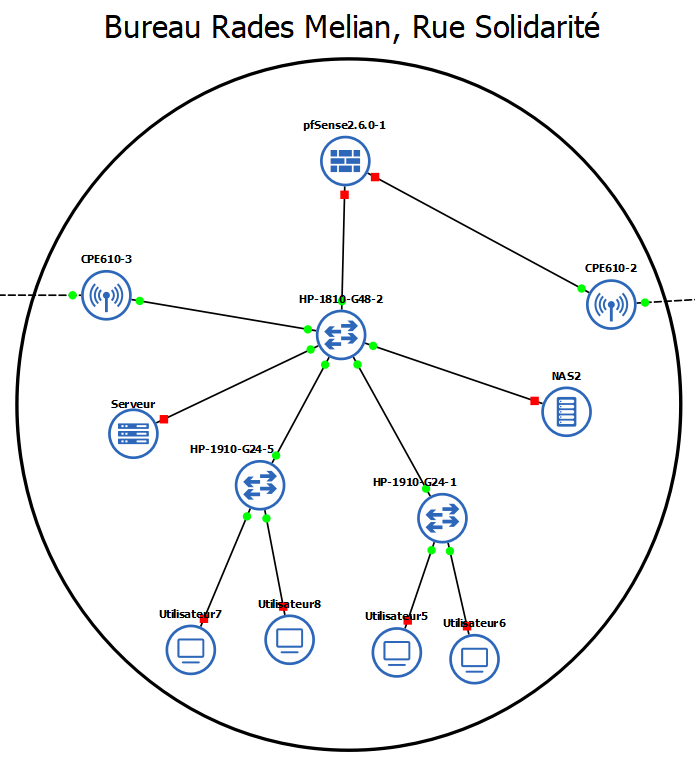
\includegraphics[width=15cm]{Images/BRadesMelian-Topologie.png}
\caption{Topologie de réseau en Rades Melian en GNS3}
\label{Chap2.4.1}
\end{figure}    
\smallskip

Dans cette figure \ref{Chap2.4.1}, nous montrons que c'est la même structure que nous avons déjà implémentée dans le bureau de Rades, mais avec le changement que nous avons ajouté le pfSense pour plus de sécurité à la branche principale.

\subsection{Configuration dans GNS3}


Dans le Chapitre 3, nous montrons le démarche que nous avons suivi pour installer pfSense et pour le moment on montre ce que Nous avons configuré les adresses IP pour les interfaces em1 et em0, comme indiqué dans les figures \ref{Chap2.4.10} à \ref{Chap2.4.12} ci-dessous, pour permettre l'accès à Internet à partir du routeur du bureau de Rades.  \\


\begin{figure}[H]
 \centering
    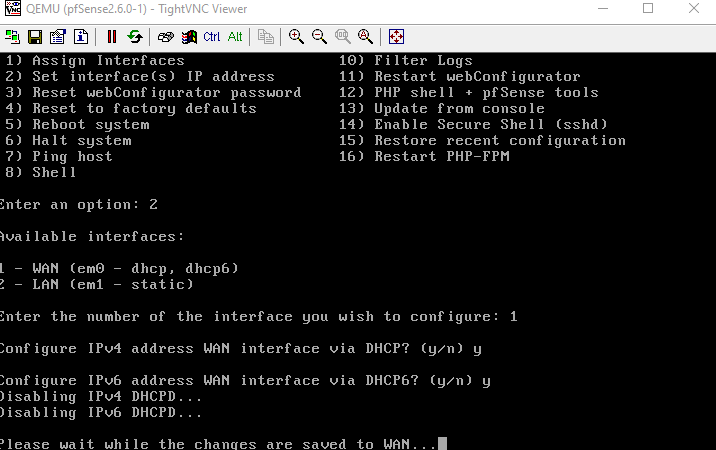
\includegraphics[width=15cm]{Images/BRadesMelian-Topologie9.png}
    \caption{Configuration du pfsense}
    \label{Chap2.4.10}
\end{figure}    
\smallskip

\begin{figure}[H]
 \centering
    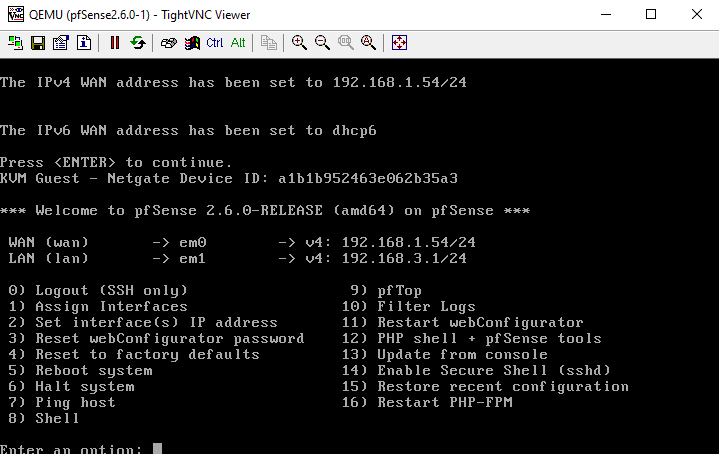
\includegraphics[width=15cm]{Images/BRadesMelian-Topologie10.png}
    \caption{Configuration du pfsense 2}
    \label{Chap2.4.11}
\end{figure}    
\smallskip

\begin{figure}[H]
 \centering
    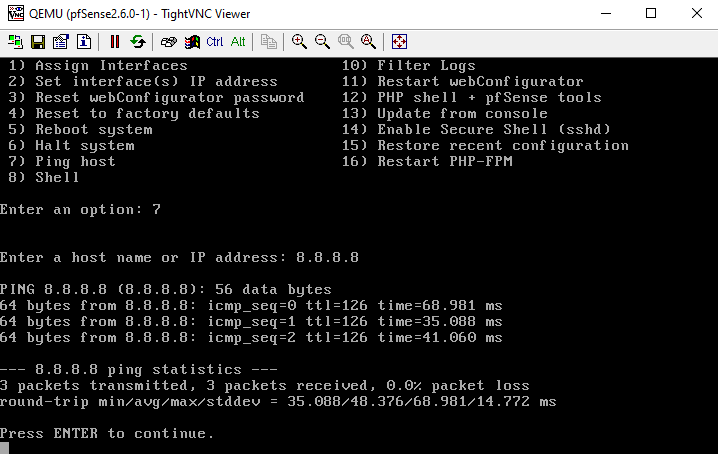
\includegraphics[width=15cm]{Images/BRadesMelian-Topologie11.png}
    \caption{Configuration du pfsense 3}
    \label{Chap2.4.12}
\end{figure}    
\smallskip


Et la résultat dans la figure \ref{Chap2.4.13} et \ref{Chap2.4.14} montre que les machines dans le réseau du Bureau Rades Melian peut accéder a l'Internet du bureau Rades et Ezzahara.  \\

\begin{figure}[H]
 \centering
    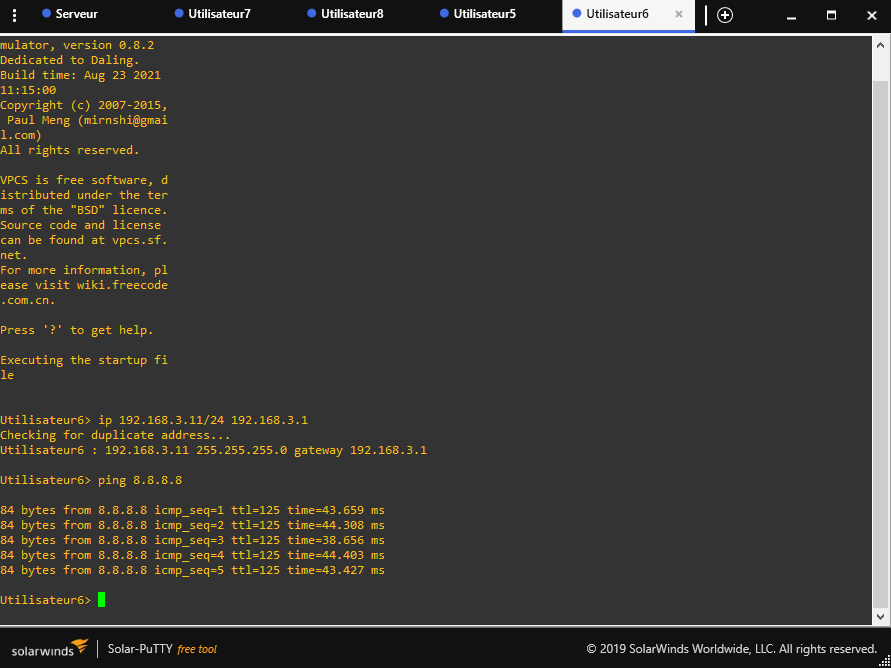
\includegraphics[width=13cm]{Images/BRadesMelian-Topologie12.png}
    \caption{Metropolitan Area Network}
    \label{Chap2.4.13}
\end{figure}    
\smallskip

\begin{figure}[H]
 \centering
    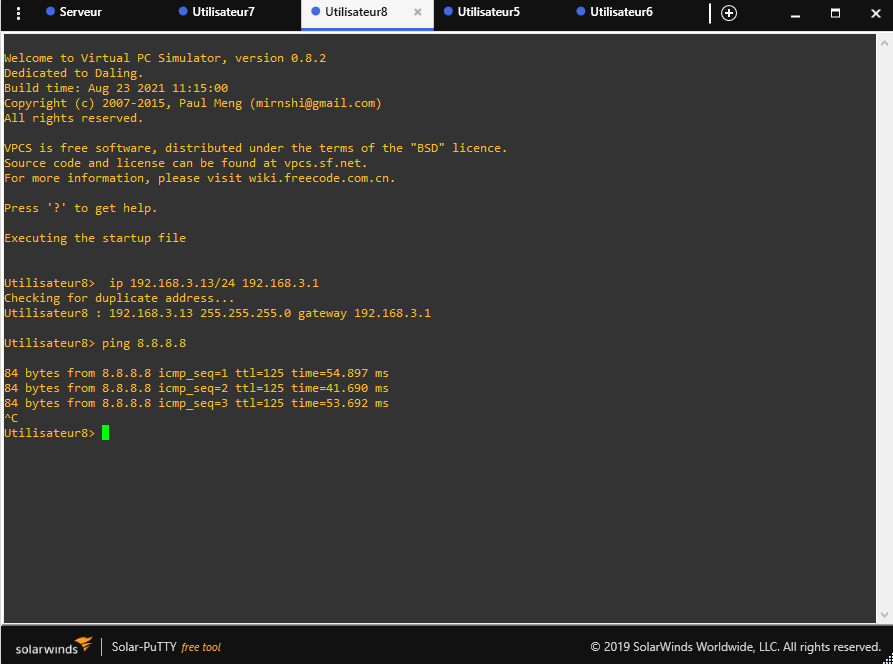
\includegraphics[width=13cm]{Images/BRadesMelian-Topologie13.png}
    \caption{Metropolitan Area Network}
    \label{Chap2.4.14}
\end{figure}    
\smallskip

\subsection{Implémentation}




La figure \ref{Chap2.4.21} montre la distance entre le Bureau Rades Melian et Rades est d'environ 1,268 km.  \\ 


\begin{figure}[H]
 \centering
    \includegraphics[width=15cm]{Images/distance1.png}
    \caption{La Distance entre le Bureau Rades et Rades Melian}
    \label{Chap2.4.21}
\end{figure}    
\smallskip


Cette distance est importante car elle affecte la qualité de la connexion Internet et la vitesse de transmission des données.  \\


\subsection{Définition du Pare-feu et choix de pfSense}

Un pare-feu est une composante essentielle de toute infrastructure réseau, responsable de la sécurisation du réseau en filtrant le trafic entrant et sortant. Nous avons opté pour l'utilisation de pfSense, une solution open-source réputée pour ses fonctionnalités avancées et sa fiabilité. \\

\begin{center}

\includegraphics[width=3cm]{Images/Logo-pfsense.png}
\end{center}


pfSense est une distribution de pare-feu et de routeur basée sur FreeBSD, offrant une interface graphique conviviale et de nombreuses fonctionnalités de sécurité. En choisissant pfSense, nous avons pu bénéficier d'une solution robuste et personnalisable pour répondre à nos besoins spécifiques.

\subsection{Implémentation du Pare-feu}

Pour déployer pfSense en tant que pare-feu dans notre infrastructure, nous avons suivi les étapes d'installation suivantes :

Nous avons utilisé la boîte E-Wall Firewall comme hôte pour notre déploiement de pfSense. \\


Nous avons procédé à l'installation de pfSense sur la boîte E-Wall Firewall en suivant les étapes décrites ci-dessous : \\

\begin{figure}[H]
\centering
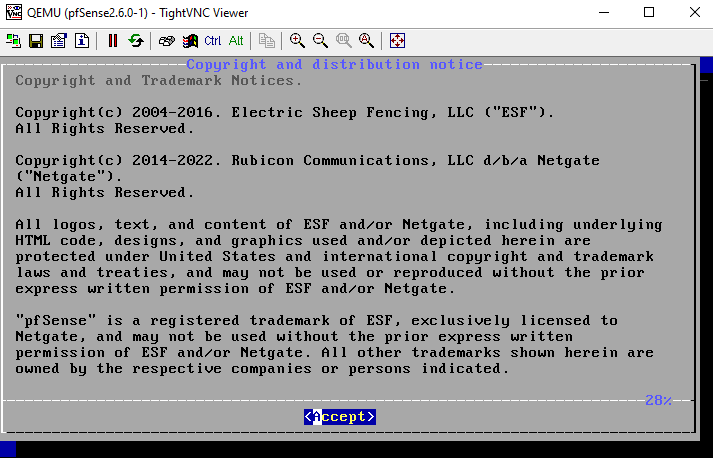
\includegraphics[width=15cm]{Images/BRadesMelian-Topologie2.png}
\caption{Installation de pfSense - Étape 1}
\label{Chap3.3.2}
\end{figure}

\begin{figure}[H]
\centering
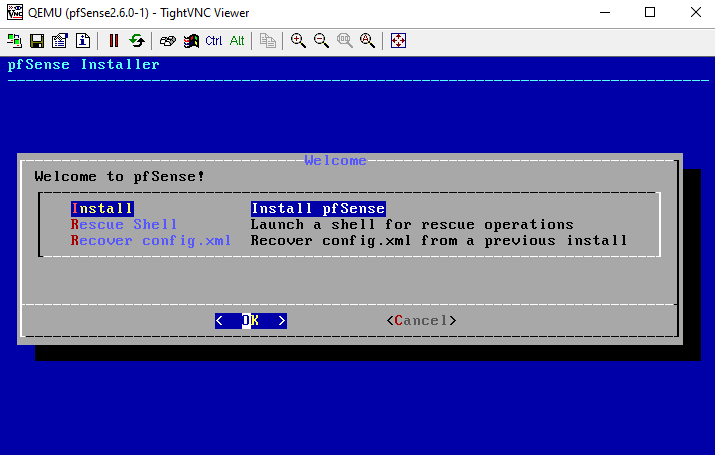
\includegraphics[width=15cm]{Images/BRadesMelian-Topologie3.png}
\caption{Installation de pfSense - Étape 2}
\label{Chap3.3.3}
\end{figure}

\begin{figure}[H]
\centering
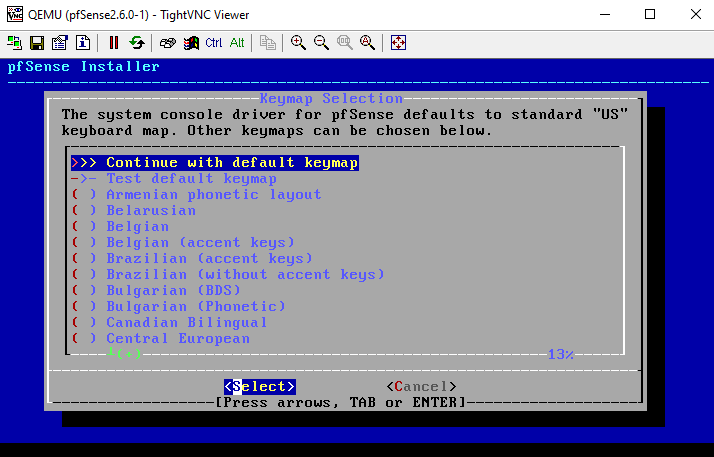
\includegraphics[width=15cm]{Images/BRadesMelian-Topologie4.png}
\caption{Installation de pfSense - Étape 3}
\label{Chap3.3.4}
\end{figure}

\begin{figure}[H]
\centering
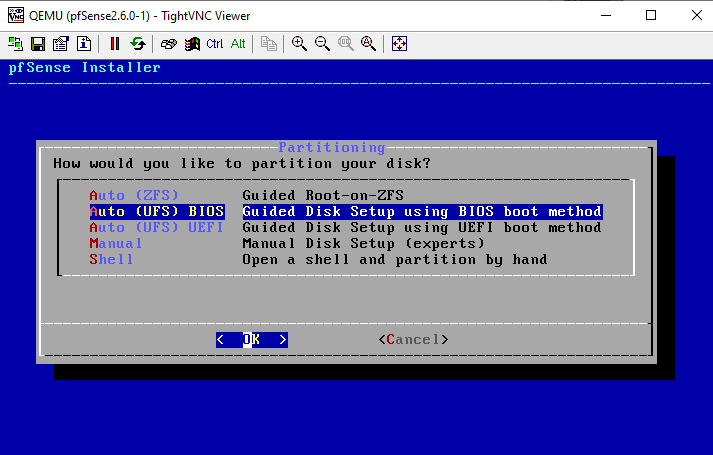
\includegraphics[width=15cm]{Images/BRadesMelian-Topologie5.png}
\caption{Installation de pfSense - Étape 4}
\label{Chap3.3.5}
\end{figure}

\begin{figure}[H]
\centering
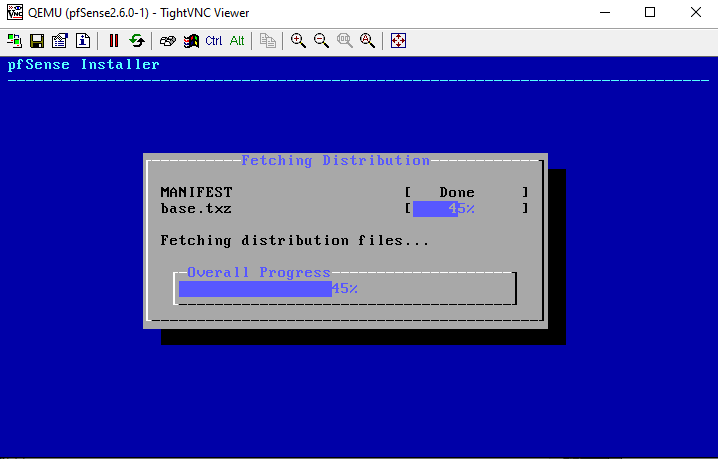
\includegraphics[width=15cm]{Images/BRadesMelian-Topologie6.png}
\caption{Installation de pfSense - Étape 5}
\label{Chap3.3.6}
\end{figure}

\begin{figure}[H]
\centering
\includegraphics[width=15cm]{Images/BRadesMelian-Topologie7.png}
\caption{Installation de pfSense - Étape 6}
\label{Chap3.3.7}
\end{figure}

\begin{figure}[H]
\centering
\includegraphics[width=15cm]{Images/BRadesMelian-Topologie8.png}
\caption{Installation de pfSense - Étape 7}
\label{Chap3.3.8}
\end{figure}

\begin{figure}[H]
\centering
\includegraphics[width=15cm]{Images/BRadesMelian-Topologie14.png}
\caption{Tableau de bord de pfSense}
\label{Chap3.3.9}
\end{figure}

\begin{figure}[H]
\centering
\includegraphics[width=15cm]{Images/BRadesMelian-Topologie15.png}
\caption{Interfaces de pfSense}
\label{Chap3.3.10}
\end{figure}

Une fois l'installation terminée, nous avons accédé au tableau de bord de pfSense pour configurer les interfaces réseau, les règles de pare-feu et d'autres paramètres de sécurité nécessaires pour protéger notre infrastructure.

pfSense offre une gamme d'options de configuration avancées, notamment la gestion des interfaces, les règles de pare-feu, les services VPN, la surveillance du trafic, etc. En utilisant ces fonctionnalités, nous avons pu personnaliser notre pare-feu pour répondre à nos exigences spécifiques de sécurité et de réseau.


\section{L'architecture Réseau Ezzahra}


Dans cette section nous présentons la topologie en GNS3 puis sa configuration et implémentation en Ezzahra.


\subsection{Topologie en GNS3}


\begin{figure}[H]
 \centering
    \includegraphics[width=15cm]{Images/BEzzahra-Topologie.png}
    \caption{Topologie Réseau Bureau Ezzahra}
    \label{Chap2.5.1}
\end{figure}    
\smallskip

Dans cette figure \ref{Chap2.5.1}, nous montrons que c'est la même structure que celle que nous avons déjà implémentée dans le bureau de Rades, mais avec la modification que nous avons ajouté une source Internet supplémentaire à notre réseau au cas où l'Internet de Rades serait coupé ou interrompu.


\subsection{Configuration en GNS3}

La configuration du réseau pour ce projet est similaire à celle du réseau du Bureau Rades. Nous avons mis en place une connexion directe avec Topnet pour assurer une connexion Internet de secours, et avons également mis en place une liaison (voir section MAN) avec les autres bureaux pour une meilleure gestion des données de l'entreprise. \\

Cette configuration permettra aux ingénieurs de travailler plus efficacement et de manière plus collaborative, en assurant une connectivité fiable et une gestion des données cohérente. \\





\subsection{Implémentation}


Les figures \ref{Chap2.5.4} et \ref{Chap2.5.5} du TP-Link installé montre la distance entre le Bureau Rades Melian et Rades est d'environ 2,843 km.  \\ 


\begin{figure}[H]
 \centering
    \includegraphics[width=15cm]{Images/152014.png}
    \caption{Distance entre Bureau Rades et Bureau Ezzhara}
    \label{Chap2.5.4}
\end{figure}    
\smallskip

\begin{figure}[H]
 \centering
    \includegraphics[width=15cm]{Images/Distance2.png}
    \caption{Distance entre Bureau Rades et Bureau Ezzhara}
    \label{Chap2.5.5}
\end{figure}    
\smallskip


\section{Conclusion}

En conclusion, la mise en place de l'infrastructure informatique pour le Mémoire De Mastère de Zeta Engineering a nécessité une analyse approfondie des besoins de l'entreprise et une sélection rigoureuse des outils et technologies utilisés pour assurer une infrastructure robuste et sécurisée. Les différentes architectures réseau mises en place ont été détaillées, du réseau local à celui du réseau MAN, en passant par les différentes implantations pour les bureaux Rades Melian et Ezzahra. \\

\begin{figure}[H]
 \centering
    \includegraphics[width=13cm]{Images/DistanceTotal.png}
    \caption{Distance Total entre les bureaux}
    \label{Chap2.6.0}
\end{figure}    
\smallskip

En somme, ce chapitre a permis de détailler les différentes étapes du déploiement de l'infrastructure IT pour le projet Mémoire De Mastère de Zeta Engineering et de présenter une approche complète et rigoureuse pour répondre aux besoins de l'entreprise tout en garantissant la sécurité et la robustesse de l'infrastructure.  \\


